%%%%%%%%%%%%%%%%%%%%%%%%%%%%%%%%%%%%%%%%%%%%%%%%%%%%%%%%%%%%%%%%%%%%%%%%%%%%%%%%%%%%%%%%%%%%%%%%%%%%%
%
%   Version     : 2.0
%
%   Filename    : main.tex
%
%   Description : This is the main file for the LaTeX thesis proposal document template.
%                 The template is intended for use by BSCS students. 
%
%                It is assumed that you can learn how to use LaTeX on your own.
%                Please check/read the following online LaTeX book:
%
%                                 http://en.wikibooks.org/wiki/LaTeX
%     
%   Author      : Florante R. Salvador
%
%   Contributors: 1.  Karlo Campos 
%                     a. margin settings for DLSU thesis paper 
%   
%   Notes       : Please email florante.salvador@dlsu.edu.ph for comments, suggestions, ideas etc.
%
%   Reference:
%
%
%   History/Updates:
%      March 12, 2009 -- created version 1.0 for release to CSC701M (Methods of Research) students
%      May 30, 2009   -- updated Title page and Abstract for undergrad ST students
%
%      Feb 27, 2015 -- Created Version 2 (major overhaul): changed class to report, created a figures folder, 
%                               removed unnecessary packages, added new comments  based on Ethel Ong's slides
%
%%%%%%%%%%%%%%%%%%%%%%%%%%%%%%%%%%%%%%%%%%%%%%%%%%%%%%%%%%%%%%%%%%%%%%%%%%%%%%%%%%%%%%%%%%%%%%%%%%%%%%
\documentclass[12pt,titlepage,onepage, letterpaper]{report}





%
%-- specify related packages
%

%
% \usepackage[utf8x]{inputenc}
%

\usepackage{apacite}           %-- APA style citation 
                               %-- refer to http://www.ctan.org/tex-archive/biblio/bibtex/contrib/apacite/

%
%  \usepackage{ucs}
%

\usepackage{changepage}

\usepackage{amsmath}           %-- American Math Society packages
\usepackage{amsfonts}
\usepackage{amssymb}

\usepackage{float}


\usepackage{graphicx}          %-- graphicx package needed for including figures in JPG or PNG format
 
%
%\usepackage{graphics}          %-- graphics related package (this was commented out) use when image is in EPS format
%

\usepackage{verbatim}          %-- this package allows you to have multiple lines of comments by
                               %-- example:
                               %   \begin{comment}
                               %        ...your text here...
                               %   \end{comment}  

\usepackage{color}             %-- allows use of color with text
                               %-- example:  \textcolor{red}{This is the colored text in red.}

\usepackage{url}  %-- allows use of URLs example: \url{https:\ccs1.dlsu.edu.ph}
% Added packages by team
\usepackage{booktabs}          %-- package from JASP statistics tool
\usepackage{pdfpages}          %-- allows use of PDF files in document
\usepackage{subcaption}
\usepackage[utf8x]{inputenc}
\usepackage{breakurl}
\renewcommand{\UrlFont}{\normalfont}

%
%-- set margins,  you may need to edit this for your own printer
%
\topmargin 0.0in
\oddsidemargin 0.0in
\evensidemargin 0.0in

\voffset 0.0in
\hoffset 0.5625in

\textwidth 5.75in
\textheight 8.5in


\parskip 1em
\parindent 0.25in

\bibliographystyle{apacite}            %-- use APA citation scheme

\hyphenation{ana-lysis know-ledge}     %-- LaTeX may not hyphenate correctly some words you use in your document
                                       %-- use \hyphenation to instruct LaTeX how to do it correctly, example above

\newcommand{\degree}{^{\circ}}         %-- use \newcommand to create your own "commands"
                                       %-- \newcommand works like the #define you learned in your COMPRO1 class

\newcommand{\etal}{et al.}
\newcommand{\figref}[1]{Figure \ref{#1}}
\newcommand{\appref}[1]{Appendix \ref{#1}}

\newenvironment{subs}
  {\adjustwidth{3em}{0pt}}
  {\endadjustwidth}


\newcommand{\thestitle}[1]{{\Large \textsc{#1}}}                %-- includes LaTeX source file for the preamble 
                                  %-- include packages, sets the margin sequence, and many more... 
                                  %-- your job: check if the settings are suitable for your own printer
\begin{document}
\graphicspath{{figures/}}  %-- figures is the name of the folder containing images JPG or PN



%%%%%%%%%%%%%%%%%%%%%%%%%%%%%%%%%%%%%%%%%%%%%%%%%%%%%%%%%%%%%%%%%%%%%%%%%%%%%%%%%%%%%%%%%%%%%%%%%%%%%%
%
%   Filename    : title_page.tex 
%
%   Description : This file will contain your Title Page.
%                 
%%%%%%%%%%%%%%%%%%%%%%%%%%%%%%%%%%%%%%%%%%%%%%%%%%%%%%%%%%%%%%%%%%%%%%%%%%%%%%%%%%%%%%%%%%%%%%%%%%%%%%

\begin{titlepage}
\centering


%-- **EDIT** the following line to indicate your thesis title
\thestitle{Development of a Game-Based Learning Environment for Senior High School Precalculus following an Outcomes-Based Methodology}

\vspace{1.75cm}
A Thesis Proposal\\
Presented to\\
the Faculty of the College of Computer Studies\\
De La Salle University Manila

\vspace{1.75cm}
In Partial Fulfillment\\
of the Requirements for the Degree of\\
Bachelor of  Science in Computer Science

\vspace{1.75cm}
by\\
%-- **EDIT** the following line to indicate your name 
\vspace{1cm}

DIONISIO, Geryco Eugynn \\
OLIQUINO, Alfred B.  \\
RANJO, Joshua Aaron P.  \\
SILVERIO, Gwyneth Alysson P.  \\

\vspace{1.75cm}
%-- **EDIT** the following line to indicate your adviser's name 
Ryan Samuel DIMAUNAHAN \\
Adviser

\vspace{1.75cm}
\today
\end{titlepage}
              %-- includes LaTeX source file for the Title Page 
                                  %-- your job: **EDIT THIS FILE ** to indicate your own title, name, and thesis adviser's name


%%%%%%%%%%%%%%%%%%%%%%%%%%%%%%%%%%%%%%%%%%%%%%%%%%%%%%%%%%%%%%%%%%%%%%%%%%%%%%%%%%%%%%%%%%%%%%%%%%%%%%
%
%   Filename    : abstract.tex 
%
%   Description : This file will contain your abstract.
%                 
%%%%%%%%%%%%%%%%%%%%%%%%%%%%%%%%%%%%%%%%%%%%%%%%%%%%%%%%%%%%%%%%%%%%%%%%%%%%%%%%%%%%%%%%%%%%%%%%%%%%%%

\begin{abstract}

During the 2018 and 2022 Programme for International Student Assessment (PISA) by the Organization for Economic Co-operation and Development (OECD), the Philippines placed low in the rankings, especially in mathematics. A subject in which focus and attention are needed, teaching mathematics to students seems to have become a challenging task in itself by not losing the interest of the students, a task in which video games usually excel. Video games have a long history of being used mainly for entertainment purposes, but the educational application of this technology is becoming well known as well. Educational games are the fruit of utilizing video game technology in pursuit of the improvement of the quality of education. Bringing out the positive benefits of video games to support a person’s learning development is the main goal of educational games. Game-based learning makes use of the positive benefits of educational games to support learning outcomes.  This paper aims to design, develop, and evaluate a game-based learning environment that could assist in teaching a Precalculus concept in the form of Conic Sections, a subject involving Analytical Geometry.

%
%  Do not put citations or quotes in the abract.
%

%Keywords can be found at \url{http://www.acm.org/about/class/class/2012?pageIndex=0}.  Click the 
%link ``HTML'' in the paragraph that starts with ''The \textbf{full CCS classification tree}...''.

\begin{flushleft}
\begin{tabular}{lp{4.25in}}
\hspace{-0.5em}\textbf{Keywords:}\hspace{0.25em} & Education, Game-Based Learning, Serious Games, Precalculus, etc.\\
\end{tabular}
\end{flushleft}
\end{abstract}
                %-- this is the Abstract page
                                  %-- your job: **EDIT THIS FILE** to indicate your own abstract

\pagenumbering{roman}             %-- this will number pages as i, ii, iii, etc...
\setcounter{page}{2}

\tableofcontents                  %-- this command is used to generate the Table of Contents


\newpage
\listoffigures                    %-- this command is used to generate List of Figures

\newpage                       
\listoftables                     %-- this command is used to generate List of Tables

\newpage

\pagenumbering{arabic}            %-- this will number pages as 1, 2, 3, etc...
\setcounter{page}{1}              


%%%%%%%%%%%%%%%%%%%%%%%%%%%%%%%%%%%%%%%%%%%%%%%%%%%%%%%%%%%%%%%%%%%%%%%%%%%%%%%%%%%%%%%%%%%%%%%%%%%%%%
%
%   Filename    : chapter_1.tex 
%
%   Description : This file will contain your Research Description.
%                 
%%%%%%%%%%%%%%%%%%%%%%%%%%%%%%%%%%%%%%%%%%%%%%%%%%%%%%%%%%%%%%%%%%%%%%%%%%%%%%%%%%%%%%%%%%%%%%%%%%%%%%

\chapter{Research Description}
\label{sec:researchdesc}    %--note: labels help you with hyperlink editing (using your IDE)

\section{Background of the Study}
Games in the form of digital display, video games have been around nearly as old as the early development of the first computers. In October of 1958, Physicist  William Higinbotham created what is believed to be the very first video game, a very simple game of tennis but in the form of an electronic display, controlling the ‘rackets’ up-and-down with a knob to hit the bouncing ball on the screen. Higinbotham spent two weeks planning and creating the device for the game, and after some debugging, the very first video game debuted with the name Tennis for Two (American Physical Society, 2008). Video games are often made for the main purpose of entertainment as a form of recreational activity. However, by definition, a video game is the mode of interaction between a player, or a group of players, and a machine with the help of an electronic display, which follows a “meaningful fictional context,” and establishes an emotional attachment between the players and the results of their actions within the fictional context (Bergonse, 2017). Nowadays, there are a wide range of video games available. Ranging from different genres such as role-playing games (RPGs), first-person shooters (FPS) games, fighting games, and many others. \figref{fig:moderngames} shows some of the most popular games today including League of Legends, Dota 2, and Counter-Strike: Global Offensive.

%--- the following example shows how to include a figure in PNG format
\begin{figure}[h]                %-- use [t] to place figure at top, [b] to place at the bottom, [h] for here
   \centering                    %-- use this to center the figure
   
\includegraphics{moderngames.png}      %-- include image file named as "disneychart.png" 
   \caption{Some of the modern video games}
    \label{fig:moderngames}
\end{figure}


But other than for entertainment purposes, video games are also often used for different purposes such as educational and training applications. According to Mestadi (2018), serious games can be described as having the property of: a game, a mental contest, an interactive computer application, a digital game, a simulation, a virtual environment, a mixed reality/media. All of these being applied for different purposes in serious fields such as education, health, and government/corporate training. Serious games are the kind of video games that are made with the purpose of imparting specific beneficial effects to the users while using the fun elements of the game to keep the users engaged in the activity. Some aviation companies such as the Gleim Aviations offer flight training courses that utilize serious games such as their X-Plane flight training course, the training includes different pilot trainings for flight lessons, and also a flight simulation with the help of the ultra-realistic X-Plane flight simulator (Gleim Aviation, 2021). As shown in Figure 2, X-Plane flight simulator provides trainees a similar experience of flying an actual airplane with the help of excellent graphics, great flight models, and different sorts of realistic scenarios replicated in the simulation.

\begin{figure}[h]
   \centering                    
   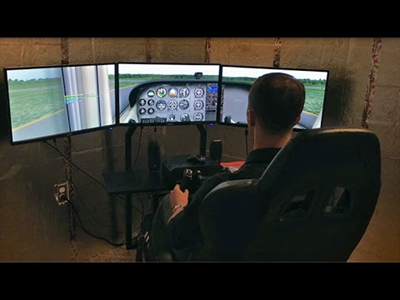
\includegraphics{flighttraining.png}
   \caption{Gleim X-Plane Flight Training Course Demonstration}
    \label{fig:flighttraining}
\end{figure}

Meanwhile, the application of serious games in the field of education has already been explored. This development did not come as a surprise since the purpose of developing serious games is to be used for educational purposes rather than entertainment. According to a meta-analysis conducted by Yu Zhongen (2018), one of the reasons why serious games are effective as a tool for education is because of its impact on the learners’ mood towards learning as an activity in this form of a game. An example of this educational serious game is Treefrog Treasure (n.d.), as shown in Figure 3. This is a type of platformer game developed for kids in the level of primary or elementary education. The goal of this game is to teach kids the concept of whole numbers, fractions, and percentages.

\begin{figure}[h]
   \centering                    
   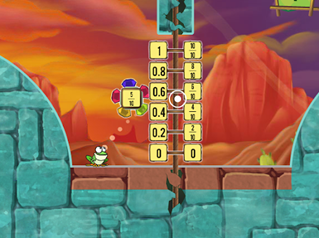
\includegraphics{treefrogtreasure.png}
   \caption{Treefrog Treasure}
    \label{fig:treefrogtreasure}
\end{figure}

When it comes to what makes a good serious game for teaching, Shute and Ke (2012) have synthesized their findings and derived seven core components of a well-designed serious game. Some of the derived components include:  Interactive problem solving, Specific goals/rules, adaptive challenges, ongoing feedback, and sensory stimuli. It is with these components that make a serious game provide an environment that promotes learning. In the study by Hassen Ben Rebbah (2019), they have shown that serious games have the potential to provide and/or promote intrinsic motivation of learners, situated learning, and learning from mistakes.

In global assessments for mathematics achievement, the Philippines has consistently ranked as one of the lowest in comparison to other countries. In 2018, the Philippines participated in the Programme for International Student Assessment (PISA) of the Organization for Economic Co-operation and Development (OECD), a triennial international assessment administered to 15-year old  learners, who are near the end of their compulsory basic education (Department of Health, n.d.). Released on the 3rd of December 2018, the PISA results revealed that Filipino students achieved an average score of 353 in Mathematical Literacy, which was significantly lower than the OECD average of 489 points. In addition to this, only 19.7 percent of Filipino students attained at least the minimum proficiency level in Mathematical Literacy.

Precalculus, a mathematics subject offered in Senior High School (SHS), is perceived to be difficult due to its concepts relying on formal definitions and proofs. In 2019, a study was conducted by Jaudinez in order to explore the teaching of SHS mathematics in the Philippines, and the results revealed that there were a number of problems when teaching precalculus to students. The identified problems include: lack of teaching strategies for difficult topics, lack of instructional resources, and lack of performance-based activities. Difficult topics were not abundantly reinforced, which caused teaching to be heavily dependent on the traditional way. Furthermore, lessons lack performance-based activities and tasks, and only conclude with practice exercises and tests. All the problems listed prior are factors to the low performance of students in procedural knowledge, computational skills, visualization, problem solving and other skills and processes in mathematics.

In order to design and develop a GBLE to target specific LOs in an educational game development, an Outcomes-Based Methodology could be followed (Sison et al, 2018). As Figure 4 shows, the first step in the GBLE development would involve identification of the LOs, followed by determining the genre of the game to be developed. After these two steps, the writing of the premise of the game would then be prioritized. This premise should clearly answer these three questions: (1) what is the player’s goal?, (2) how will the player achieve that goal?, and (3) what is the environment or world where the players will achieve the said goal? After this step, the next one would include designing the LO mechanics to be used as a game mechanic that would help the player-learners. This step is divided into achieving an LO, and then determining whether or not the LO has been achieved, and to what extent. This step involving the designing of the LO mechanics would repeat as long as it needs to take to completely build the GLE after the repeated designing and evaluation of the LO mechanics and related elements of it. The loop in the incremental development of the GLE might sometimes include a redesign for an LO mechanic based on its performance evaluation on the playtesting. Following this part of the methodology would include the integration of all the elements before proceeding to the final playtest and evaluation of the GBLE.

\begin{figure}[h]
   \centering                    
   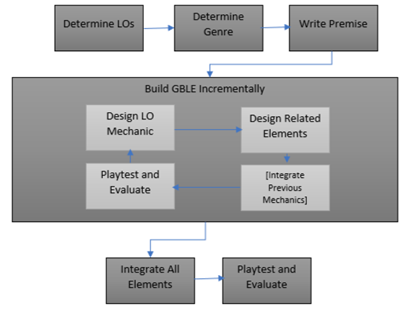
\includegraphics{outcomebased.png}
   \caption{Outcome-Based Methodology for Game-Based Learning Environment Development}
    \label{fig:outcomebased}
\end{figure}

The Philippines has constantly been placed among the lowest ranks in multiple indices regarding mathematics achievement. In the PISA 2018, students scored significantly lower than the OECD average, and in the Trends in International Mathematics and Science Study 2019 (TIMSS), the Philippines scored the lowest among all 58 participating countries (Magsambol, 2020). According to Jaudinez (2019), there were several problems when precalculus was being taught to students as revealed in his study in exploring the teaching of SHS Mathematics in the Philippines. One of the problems that were identified is the lack of teaching strategies for difficult topics. Teaching is heavily dependent on the traditional face to face method, and difficult topics were not reinforced causing students to have difficulty in learning and lose interest in the subject. In addition to this, although the Philippines has already adapted the outcomes-based education approach in schools, the outcomes-based methodology still has not been applied to the design and development of a SHS precalculus GBLE.

\section{Research Objectives}
\label{sec:researchobjectives}

In this section, we define the research objectives that guide this thesis. These objectives serve to focus the study, providing clear goals that aim to address the research questions posed. This thesis aims to achieve the following objectives:

\begin{subs}
\subsection{General Objective}
\label{sec:generalobjective}

To design, develop, and evaluate a Game-Based Learning Environment (GBLE) that supports in teaching Senior High School (SHS) Precalculus pedagogy. The GBLE will be evaluated for its ability to support the achievement of select learning outcomes of the said subject, as well as for its ability to engage player-learners.

\subsection{Specific Objectives}
\label{sec:specificobjectives}

The specific objectives for this study are as follows:

\begin{enumerate}
   \item To review challenges in Senior High School (SHS) Precalculus pedagogy;
   \item To identify target learning outcomes (LO) from SHS Precalculus;
   \item To design LO mechanics that support the achievement of the target LOs identified;
   \item To develop a Game-Based Learning Environment (GBLE) incorporating the LO mechanics identified; and
   \item To determine the effects of the GBLE in terms of supporting the achievement of the target LOs and the engagement of player-learners
\end{enumerate}
\end{subs}

\section{Scope and Limitations of the Research}
\label{sec:scopelimitations}

The goal of the study is to design, develop and evaluate a game-based learning environment (GBLE) that  would support senior high school precalculus pedagogy. The GBLE to be developed is intended to support the achievement of selected precalculus Learning Outcomes (LOs). Thus, player-learners are to play the GBLE while they are taking the topics covered by the selected LOs. It is not meant to introduce topics, nor is it meant to serve as an assessment tool for SHS Precalculus.

\begin{subs}
\subsection{Challenges in Senior High School Precalculus Pedagogy}
In order to identify challenges in SHS Precalculus Pedagogy, a literature review would be conducted. This literature review would include data from the Philippines as well as its neighboring countries in South East Asia (SEA). It is hoped that other Southeast Asian countries may have similar educational contexts as in the Philippines, and may have similar challenges. In the absence of enough data to identify pedagogical challenges, the literature review would be expanded to include other countries outside SEA that may have the same educational contexts as the Philippines.

\subsection{Learning Outcomes of Precalculus}
In order to identify target LOs from SHS Precalculus, the 2019 SHS Curriculum Guide (SHS-CG) from the Department of Education (DepEd) would be reviewed. In addition, a SHS Precalculus context expert would be consulted. Identifying LOs will be time consuming because the process should be as thorough as possible for there are things to be considered. In choosing LOs, the difficulty of the topics in the curriculum, the need of assistance from a third party for certain topics, and how applicable the development of GBLE will be for the LOs should all be considered first before deciding which LOs should be used. The LOs that translate the best into a GBLE, as decided upon by consultations with the context expert would be selected. Following the Outcomes-Based Methodology of Sison et al (2018), once target LOs have been identified, LO mechanics that target the LOs would be designed.

Based on the advice of the research adviser and the context expert, the chosen target LOs were chosen from the Department of Education’s curriculum guide for Senior High School STEM Course (2019). The target LOs were from the Analytical Geometry content which mainly discusses Conic Sections. The target LOs were: Learning Competency No. 14: to recognize the equation and important characteristics of the different type of conic sections, and Learning Competency No. 15: to solve situational problems involving conic sections.

\subsection{Learning Outcomes Mechanics}
In order to adhere to the aforementioned methodology, and to rapidly develop the GBLE, these LO mechanics would be integrated, playtested and evaluated periodically by the proponents of the study along with the context expert and research adviser. These LO mechanics would be part of the core gameplay loop of the GBLE. To support the LO mechanics, several non-LO mechanics may be designed, but they would not be prioritized for the study and would only be designed to support the core gameplay loop of the GBLE. The GBLE to be developed will be for desktop computers, which can run more powerful software compared to other devices such as consoles and mobile devices. Due to the transition from face-to-face classes to online classes, it is more likely that the participants will be able to undergo the experiment.

\subsection{Game-Based Learning Environment Design}
Developing the game would involve choosing a platform in which is the most available one for the player-learners. This is in consideration of the students that are at risk or vulnerable situations. Unity, a cross-platform game engine, would be used to develop the game because it has several features such as rendering, scripting, physics, and asset tracking that help reduce the time and cost for developing games. It also supports several platforms, allowing it to be easily shared between web, PC, and mobile platforms. 

Lastly, in order to determine the effect of the GBLE on the engagement and academic performance of the player-learners, a quasi-experiment would be done which involves assessing the difference in academic performance before and after the playtesting by comparing pre-test and post-test results. Only a quasi experiment will be used instead of true experimental research as there is only a limited time to gather data. Measures of statistical significance would be used in the comparison; should the desired number of n participants may be gathered, parametric tests would be used otherwise, non-parametric tests would have to be utilized.
\end{subs}

\section{Significance of the Research}
\label{sec:significance}

This study aims to develop a GBLE that would increase the engagement and academic performance of senior high school students and player-learners. Additionally, this study also aims to give instructors a new platform for teaching their students. The following individuals will benefit from this research: 

\begin{subs}
\subsection{Students}
This study can give students an alternative way of learning through the use of educational serious games. The game-based learning environment developed can be used by students as a support tool in their precalculus topics in order to further improve their knowledge and increase their motivation.

\subsection{Instructors}
This study can give instructors an alternative teaching method rather than the traditional face to face way, and the GBLE developed can be used by instructors as a support tool in teaching precalculus to their students in order to keep them more engaged in learning.

\subsection{Game Developers}
The GBLE developed can give game developers new ideas in designing and developing educational serious games, most especially in the domain of mathematics. Furthermore, game developers will be able to adapt the idea of what to prioritize first when creating games, such as focusing on the learning outcomes first before the design of the game itself.

\subsection{Future Researchers}
This study can assist future researchers given the knowledge of the processes involved when developing a GBLE. Furthermore, they will be able to use this paper as a reference for more studies related to this topic in the future.
\end{subs}

\section{Research Methodology}
The following are the sets of activities that will be performed in order to accomplish the objectives of the study:

\begin{figure}[h]
   \centering                    
   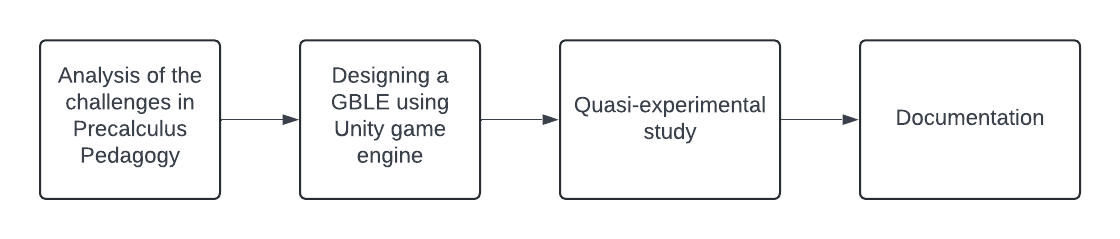
\includegraphics[scale=0.9]{studyflowchart.png}
   \caption{Step-by-step flowchart for the study}
    \label{fig:studyflowchart}
\end{figure}

\begin{figure}[h]
   \centering                    
   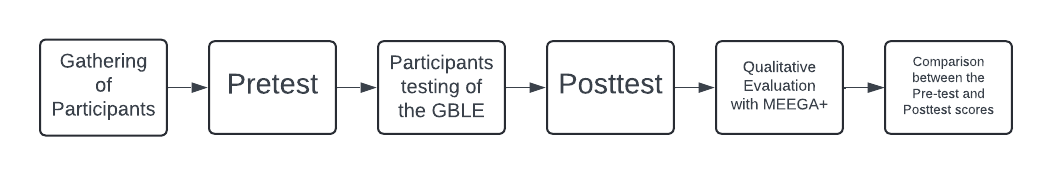
\includegraphics{quasiexperiment.png}
   \caption{Step-by-step flowchart for the Quasi-experiment}
    \label{fig:quasiexperiment}
\end{figure}

\begin{subs}
\subsection{Investigation of Precalculus Pedagogy}
Challenges in the practice of teaching Precalculus in senior high school students will be investigated. Various related works and literature will be reviewed and examined in relation to these challenges. The curriculum of SHS students for Precalculus will be observed in order to generate ideas regarding where the assistance of using GBLE would be most relevant. In addition to checking the curriculum, a SHS Precalculus professor will be consulted in order to find out the learning outcomes that students struggle with.

\subsection{Design of the GBLE}
An educational game would then be designed and developed using the Unity game engine to assist the students in learning precalculus. The game design and learning outcomes involved would be based on the gathered data and feedback from Precalculus professors and serious game developers. Before the designing of the game, the learning outcomes should first be designed in order to assess the features that will be in the game. This way, the content of the game will be centered around the important points of the LOs.

\subsection{Quasi-experimental Study}
The first process in the quasi-experiment with a one-group pretest-posttest design will be the gathering of the participants. The participants will take a pre-test assessment in order to evaluate their performance in Precalculus, and then undergo a 1 hour playtest or until game completion. The participants will then take a post-test assessment regarding their performance in Precalculus, and a survey will be conducted to measure their engageability and overall experience. When all the data has been collected, the data will be compared and will undergo statistical analysis through a paired t-test in order to determine if there is a significant difference in the pre-test and post-test scores.
Since the participants involved are all senior high school students which are mostly in the age range of 16-18 years old, appropriate consent forms would be provided for the student and their guardians. Names of the participating students would be kept confidential. All personal data that will be collected will be disposed of after being used in this study.
For the qualitative evaluation, a MEEGA+ questionnaire (2018) will be given to those students that tested the game to evaluate their feedback about their experience with the game. The test scores of two groups, and the MEEGA+ results from the game testers would be used to create a statistical analysis about the performance of the proposed GBLE.
\subsection{Documentation}
All the plans, evaluations, and implementations that were involved in this study such as the data collected and the different processes in creating a GBLE will be documented and maintained up-to-date within the duration of this study.
\subsection{Calendar of Activities}
The following tables shows the Gantt chart of the activities for 2021 and 2023:

Table \ref{tab:timetableactivities2021} and Table \ref{tab:timetableactivities2023} shows a Gantt chart of the activities.  Each bullet represents approximately one week worth of activity.

%
%  the following commands will be used for filling up the bullets in the Gantt chart
%
\newcommand{\weekone}{\textbullet}
\newcommand{\weektwo}{\textbullet \textbullet}
\newcommand{\weekthree}{\textbullet \textbullet \textbullet}
\newcommand{\weekfour}{\textbullet \textbullet \textbullet \textbullet}

%
%  alternative to bullet is a star 
%
\begin{comment}
   \newcommand{\weekone}{$\star$}
   \newcommand{\weektwo}{$\star \star$}
   \newcommand{\weekthree}{$\star \star \star$}
   \newcommand{\weekfour}{$\star \star \star \star$ }
\end{comment}

\begin{table}[h]   %t means place on top, replace with b if you want to place at the bottom
\centering
\caption{Timetable of Activities (2021)} \vspace{0.25em}
\begin{tabular}{|p{2in}|c|c|c|c|c|c|c|c|} \hline
\centering Activities (2021)            & Mar   & Apr & May & Jun & Jul & Aug & Sep \\ \hline
Review Serious Games \& Related Works   & \weekfour & \weekfour & \weekfour &  &  &  &  \\ \hline
Data Gathering for Senior High School Teaching Pedagogy    &   &  &  & \weekfour & \weekfour & \weekfour &  \\ \hline
GBLE Design      &   &  &  &  &  & \weekfour & \weekfour \\ \hline
Documentation & \weekfour  & \weekfour & \weekfour & \weekfour & \weekfour & \weekfour & \weekfour \\ \hline
\end{tabular}
\label{tab:timetableactivities2021}
\end{table}
\begin{table}[h]   %t means place on top, replace with b if you want to place at the bottom
\centering
\caption{Timetable of Activities (2024)} \vspace{0.25em}
\begin{tabular}{|p{2in}|c|c|c|c|c|c|c|} \hline
\centering Activities (2024)            & Feb & Mar & Apr & May & Jun & Jul \\ \hline
GBLE Development    & \weekfour & \weekfour & \weekfour & \weekfour & \weekfour &  \\ \hline
GBLE Testing        &   &   &   & ~~\weektwo  & \weekfour & \weekone~~~ \\ \hline
Data Collection     &   &   &   &   &   & \weektwo~~ \\ \hline
Results and Analysis&   &   &   &   &   & ~\weekone~~ \\ \hline
Documentation &  \weekfour & \weekfour & \weekfour & \weekfour & \weekfour & \weektwo~~~ \\ \hline
\end{tabular}
\label{tab:timetableactivities2023}
\end{table}

\end{subs}               %-- includes LaTeX source file for Chapter 1: Research Description
                                  %-- your job: **EDIT THIS FILE** to indicate your own research description

%%%%%%%%%%%%%%%%%%%%%%%%%%%%%%%%%%%%%%%%%%%%%%%%%%%%%%%%%%%%%%%%%%%%%%%%%%%%%%%%%%%%%%%%%%%%%%%%%%%%%%
%
%   Filename    : chapter_2.tex 
%
%   Description : This file will contain your Review of Related Literature.
%                 
%%%%%%%%%%%%%%%%%%%%%%%%%%%%%%%%%%%%%%%%%%%%%%%%%%%%%%%%%%%%%%%%%%%%%%%%%%%%%%%%%%%%%%%%%%%%%%%%%%%%%%

\chapter{Review of Related Literature}
\label{sec:relatedlit}

\section{Serious Games}
Most games are created so that people can be engaged in the content of the game, with the primary purpose of entertaining its users. However, there are games that are not limited to just entertainment, and this genre of games is called a serious game. Serious games are defined as games that do not have entertainment, enjoyment, or fun as their primary purpose, and can be distinguished from video games by their design objectives (Eid, Laamarti, \& El Saddik, 2014). According to Gamelearn (2020), the primary objective of serious games is learning or practicing a skill rather than entertainment, and serious games have been already used in several sectors such as education, science and health, and even aeronautics. Serious games are games with a main goal of helping people learn and develop skills, this could even result in behavior change of the players. The things that serious games specialize in is that they are made to be entertaining, engaging, and immersive (Roolvink, 2021). They are designed to let players solve problems in different areas and involve them in challenges and rewards while maintaining the engaging and entertaining aspects that serious games have (Roolvink, 2021). According to Thalmann (2014), most researchers' definition of a serious game is that it must have an entertainment dimension, and that a serious game has a potential to provide an immersive experience to players through multimodal interaction in different contexts such as training, health, and education.
Serious games in different sectors have been implemented and are available in several platforms such as mobile and computer. Some examples of the popular existing serious games are Microsoft Flight Simulator (1982), World Without Oil (2007), and Sea Hero Quest (2016). Microsoft Flight Simulator is a flight simulator program created for computers, wherein players can learn and practice their piloting skills in a real-time atmospheric simulation. Second, World Without Oil was an alternate reality game that lasted for 32 days, wherein the main objective is to help its players visualize what subtle and deep effects an oil crisis has in their lives, in order to call attention to a possible near-future oil shortage. Lastly, Sea Hero Quest is a mobile game released in association with Alzheimer’s Research UK as a contribution to research in dementia. People with dementia can face challenges with navigation early on, and by playing the game, reliable data on how navigational abilities can change in the healthy brain across life is provided anonymously to researchers.

\section{Precalculus Pedagogy}
\subsection{Challenges in Precalculus Pedagogy}
According to Kauffmann, Archava, Castles.., (2011), studies indicated that STEM students in the US had a 30-50\% rate of retention in engineering, and these had diverse factors including learning styles and psychological dispositions. The key factors that remained an issue in the retention of students are the poor teaching and pedagogy. The authors were also able to find out in their research according to the students’ perceptions that high school preparation is a big issue because it appears that high school mathematics barely focused on polynomial and quadratic equations in a trade off for trigonometric and exponential functions. This led to a damaging impact in pre-calculus in engineering programs.
\subsection{Unique situation of Precalculus in Philippines}
In a study by Jaudinez (2019), a number of problems were identified when it comes to teaching mathematics to senior high school students of which precalculus is specified within the study. The identified problems include the general lack of teaching strategies for difficult topics, proper teaching resources and tools, and performance-based activities. Teaching is heavily dependent on the traditional face to face method, and difficult lessons are not reinforced. The teaching of SHS mathematics started in 2016 without any references provided, and the textbooks released only a year after were not appropriate for SHS students in terms of difficulty, complexity, and context. Lastly, the lessons in precalculus lack enhancement activities or tasks that are performance-based, and only practice exercises or tests are given to the students.
\subsection{Precalculus Pedagogy Frameworks in SHS}
When it comes to the pedagogies used in the curriculum created by DepEd, they are required to use pedagogical approaches that are constructivist, inquiry-based, reflective, collaborative and integrative. As stated by the context expert, DepEd provided a way to assess learners and to determine what should be expected of them. According to the DepEd Order 8, s. in 2015, schools shall consider three (3) basic assessment criteria: written works (WW),  performance tasks (PT), and quarterly assessments (QA). In terms of teaching strategies implemented, teachers have the freedom to select which strategy, technique, However, due to the on-going nature of the Global Pandemic of COVID-19, DepEd adapted the implementation of Blended Learning.
\subsection{Blended Learning during the COVID-19 Pandemic}
According to an official statement of DepEd on 8th of June 2020, a direct order from President Duterte was issued to postpone face-to-face classes and thus the groundwork for blender learning was paved. Making use of radio, television, online and modular learning which are pre-existing methods already but are now being prepared and updated to match the needs for the current situation. Meanwhile, teachers were also being introduced and trained on how to use newer platforms and innovative tools to help them adjust in teaching in a new environment.

\section{Game-based Learning}
Game-based learning is a trend that has been implemented in several different areas, one of these being education. According to Trybus (2014), game-based learning refers to the borrowing of certain gaming principles and applying them to real-life settings to engage its users. It is a type of game play with specific learning objectives and outcomes, with a design process that involves balancing the need to cover the subject matter with the desire to prioritize gameplay (Homer, Plass \& Kinzer, 2015). EdTechReview (2013) states that game-based learning is a type of game play that includes learning outcomes and is designed to have a balance between the ability of the player to apply the said subject matter to the real world and subject matter with gameplay.
Several game-based learning environments have been implemented in different domains in order to improve the learning achievement and motivation of students. In a study by Stiller and Schworm (2019), a game-based learning environment was implemented in the domain of science and english using a game called CellCraft in order to assess the effects of gameplay on motivation, cognitive load, and performance. Results of this study showed that gaming improved the knowledge of the students and reduced their cognitive load, enabling the students to focus on their learning. Another implementation of a game-based learning environment was done in the domain of American Sign Language (ASL) by Kamnardsiri, Hongsit, Khuwuthyakorn, and Wongta (2017) in order to explore the effectiveness of the usability of the intelligent game-based system for learning ASL. The results of this study showed a significant difference in the post-test scores for the game-based learning group and the group learning using the traditional face to face method, the scores of the gaming group being higher. In addition to this, the system also engaged the students to concentrate on ASL vocabularies and gave them a sense of control and concentration while playing the game.


















               %-- includes LaTeX source file for Chapter 2: Review of Related Literature
                                  %-- your job: **EDIT THIS FILE** to indicate your review of related literature 

%%%%%%%%%%%%%%%%%%%%%%%%%%%%%%%%%%%%%%%%%%%%%%%%%%%%%%%%%%%%%%%%%%%%%%%%%%%%%%%%%%%%%%%%%%%%%%%%%%%%%%
%
%   Filename    : chapter_3.tex 
%
%   Description : This file will contain your Research Methodology.
%                 
%%%%%%%%%%%%%%%%%%%%%%%%%%%%%%%%%%%%%%%%%%%%%%%%%%%%%%%%%%%%%%%%%%%%%%%%%%%%%%%%%%%%%%%%%%%%%%%%%%%%%%

\chapter{Theoretical Framework}
\begin{comment}
This chapter lists and discusses the specific steps and activities that will be performed by the proponent to accomplish the project. 
The discussion covers the activities from pre-proposal to Final Thesis Writing.  It also includes an initial discussion on the theoretical framework to be followed.
Research activities include inquiry, survey, research, brainstorming, canvassing, consultation, review, interview, observe, experiment, design, test, document, etc.  
The methodology also includes the following information:
\begin{itemize}
   \item who is responsible for the task
   \item the resource person to be contacted
   \item what will be done
   \item when and how long will the activity be done
   \item where will it be done
   \item why should be activity be done
\end{itemize}
\end{comment}

\begin{figure}[b]
   \centering                    
   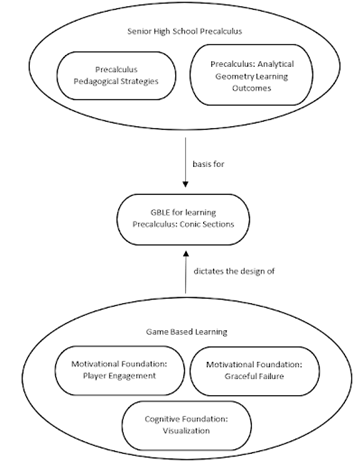
\includegraphics{theoreticalframework.png}
   \caption{Theoretical Framework}
    \label{fig:theoreticalframework}
\end{figure}

In this chapter, a theoretical framework consisting of a Game Based Learning Environment (GBLE) is used as a learning tool for precalculus pedagogy. The design of the GBLE is dictated based on three foundations, particularly player engagement,graceful failure, and visualization. The proposed GBLE uses Senior High School Precalculus Pedagogical Strategies and Analytical Geometry Learning Outcomes as a backbone for targeting Conic Sections. There are several sections below to further discuss each component of the theoretical framework in more detail.

\section{Game Based Learning}
There are three foundations under the game based learning section which will be the backbone of the GBLE to be created. Specifically, these are player engagement, graceful failure, and visualization. Each of these elements are to be discussed in further detail in every subsection below.

\subsection{Motivational: Player Engagement}
According to Schoenau-Fog (2011), the engagement must be sustained in order to motivate a player to keep playing, this means that good games must be engaging enough so players would want to keep playing them. Sharek (2018) states that engagement is the willingness of a person to participate in something, and that it cannot stand alone if they are cognitively underloaded. The GBLE to be created seeks to balance the amount of cognitive engagement of the players so they will continue to want to be engaged in the game. This could be done in several ways such as giving the players challenges that are not easily attainable but at the same time achievable. Gregory, E. (2008) made use of The Experience Sampling Method (ESM) to investigate how people feel, think, and do in their lives. This information was then used to create stories that are used in video games, and these stories help in making players more engaged as the stories were based on the feelings of people that define their experience of wanting to become more engaged in tasks. With all of these elements combined as the backbone for creating GBLEs, players would become more engaged in the game, and this can increase the ability of GBLEs to be used in an educational setting.

\begin{figure}[t]
   \centering                    
   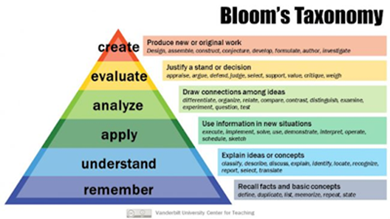
\includegraphics{bloomtaxonomy.png}
   \caption{Bloom's Taxonomy}
    \label{fig:bloomtaxonomy}
\end{figure}

According to the framework of Bloom’s Revised Taxonomy (2001), in order to assess how to develop proper learning outcomes, a hierarchy was created in order to differentiate levels of how much cognitive learning do students experience. At the top of this framework we’re the three most effective ways of cognitive learning, namely: create, evaluate, analyze. By focusing on these methods, the proposed GBLE offers learners the highest form of cognitive learning experience possible.

\subsection{Motivational Foundation: Graceful Failure}
Litts, B., \& Ramirez, D. (2014) argue that the deepest learning occurs when one fails. As failing provides an opportunity to learn from failure and further saying that learning is an iterative process of incomplete constructs and revisions which is propelled by failure. GBLEs are able to provide spaces where the consequences of failure are low, encouraging learners to take risks and try new strategies to reach their goals at their own self-regulated pace (Plass et al., 2015).

\subsection{Cognitive Foundation: Visualization}
According to Hazzard (2015), data visualization augments cognition and has different purposes such as a health bar to display a character’s status, or a skill tree showing the potential of a character. Hazzard divided data visualization used in games into two primary types: status information and training. Status information allows players to have planned choices, give players information, or both. Zammitto (2008) states that video games rely on the information players see on the screen, so if the information is not correctly visualized, it can lead to a frustrating experience for the players. Zammitto also states that a good interface is one that is not noticed. These can be included when creating GBLEs as it will be able to support the decisions that players make depending on the information they can visualize. This is especially important when GBLEs are to be used as an educational tool, as the information displayed will be very crucial in helping the players learn what the game intends for them to learn.

\section{Senior High School Precalculus}
This section contains the learning outcomes and pedagogies that will be the basis for creating a GBLE for learning Precalculus: Conic Sections. The Learning Outcomes are expected to be learned by the student players as they interact with the proposed GBLE, and the pedagogical strategies are to be used in order to have a guide in teaching Precalculus: Conic Sections through a GBLE.

\subsection{Precalculus Pedagogical Strategies}
The GBLE to be created seeks to include the strategies provided by DepEd as these pedagogies have already been used, and the efficient strategies can be used as a guide for implementing ways on how the GBLE can be used as an educational tool in helping Senior High School students learn Precalculus better. Due to DepEd's protocol for teachers to give them academic freedom to teach the way they deem appropriate for learners, there's a variety of strategies available for each individual student. But since the problem is mostly in foundation skills, most of the strategies include review of these foundational skills as well as applying such knowledge to real life situations.
\subsection{Precalculus: Analytical Geometry Learning Outcomes}
Based on the curriculum guide of DepEd for Grade 11 STEM Pre-Calculus, two LOs were chosen from the contents of Analytic Geometry through the recommendation of a Precalculus expert. The target LOs were Learning Competency 14 and 15. The first LO expects the learners to recognize the equation and important characteristics of the different types of conic sections, while the second LO expects them to solve examples of real life problems involving conic sections. To assist the player-learners in mastering these LOs would be the primary objective of the proposed GBLE for Precalculus. Both of these LOs can be targeted by a single game mechanic in the GBLE in which the players would be asked to solve puzzles in the game depicting real-world situations where the concept of Conic Sections were being applied. These puzzles would be supported with the context provided by the game’s story narration.

\section{GBLE for Learning Precalculus: Conic Sections}
The proposed GBLE for learning Precalculus Conic Sections will be using the concepts mentioned within the theoretical framework of the study. The target LOs for the Conic Sections would be the basis for how each of the GBLE’s mechanics, designs, and scenarios will be made in order for the learners to understand the concepts within the topic of Conic Sections. For example, certain learning game design principles will be followed to provide appropriate game mechanics to target the appropriate LOs by simulating real-world situations in the game where the concepts of Conic Sections should be used in order to make progress within the game. The GBLE’s goal is to provide a way for the students to learn more about the topic in a more engaging way as compared to the traditional classroom method.

               %-- includes LaTeX source file for Chapter 3: Research Methodology
                                  %-- your job: **EDIT THIS FILE** to indicate your research methodology
\chapter{Conic Lab}
\label{sec:coniclab}
\section{Game Overview}
\label{sec:gameoverview}
Conic Lab is an innovative puzzle platformer game designed with the dual purpose of engaging players and educating them on the topic of conic sections, a fundamental area of precalculus. The game consists of two doors in which the left door is where the player spawns and the right door is where the player must go through. In this game, there are several obstacles or unpassable areas where players must use the different types of conic shapes in order to assist them in passing through those situations. The game aligns with the DepEd Learning Competencies for Precalculus, specifically targeting Learning Outcomes: (14) recognize the equation and important characteristics of the different types of conic sections, and (15) solve situational problems involving conic sections. The GBLE’s target users are SHS students that are currently taking lessons on Precalculus’ Analytical Geometry: Conic Sections, on which the game could help them further understand their lessons.

\section{Software Objectives}
\label{sec:softwareobjectives}
\subsection{General Objective}
\label{sec:genobjective}
The general objective of the Game-Based Learning Environment (GBLE) is to act as a support tool for player-learners to achieve the Learning Outcomes (LOs) in Precalculus Senior High School (SHS) and at the same time while keeping them engaged through interactive and immersive gameplay experiences.

\subsection{Specific Software Objectives}
\label{sec:specsoftwareobjectives}
The specific software objectives are as follows:
\begin{enumerate}
    \item To support player-learners in achieving the target Precalculus Learning Outcomes (LOs) through the game mechanics and elements of the Game-Based Learning Environment (GBLE) as Conic Lab integrates educational puzzles and interactive tutorials which are designed to reinforce the understanding and application of conic sections,
    \item To engage player-learners through the game’s visuals, mechanics, audio, and narrative, Conic Lab offers a cutesy art style with intuitive but fairly challenging gameplay.
\end{enumerate}

\section{Scope and Limitations}
\label{sec:gamescopelimitation}
The GBLE developed is meant to be used as a support tool only, meaning that the player-learners must already have previous knowledge regarding the LOs that the GBLE will cover. The game mechanics of the GBLE are based on the LOs of Precalculus, however, it will not cover the entire subject, but rather, selected LOs in the Analytical Geometry section, specifically conic sections. The LOs used as the basis of the GBLE were chosen based on the recommendations of a Precalculus expert, as well as previous related literature.
The narrative and characters of the GBLE are entirely fictional; any similarities to actual events or persons are purely coincidental. All resources such as visuals and audio found in the game will be taken from royalty free sources. Game mechanics from already developed games and the learning game principles will serve as the basis for the game mechanics of the GBLE.

\section{Architectural Design}
\label{sec:gamearchdesign}
The architectural design for the proposed GBLE will be composed of both learning and game mechanics. The game mechanics are meant to complement each learning mechanic to improve the learning experience of the players. The Foundation and Evaluation modules consist of the learning elements and which game mechanics would be created in order to integrate them into the game for the players to experience them.

\begin{figure}[H]
\hspace*{-1cm}
   \centering                  
   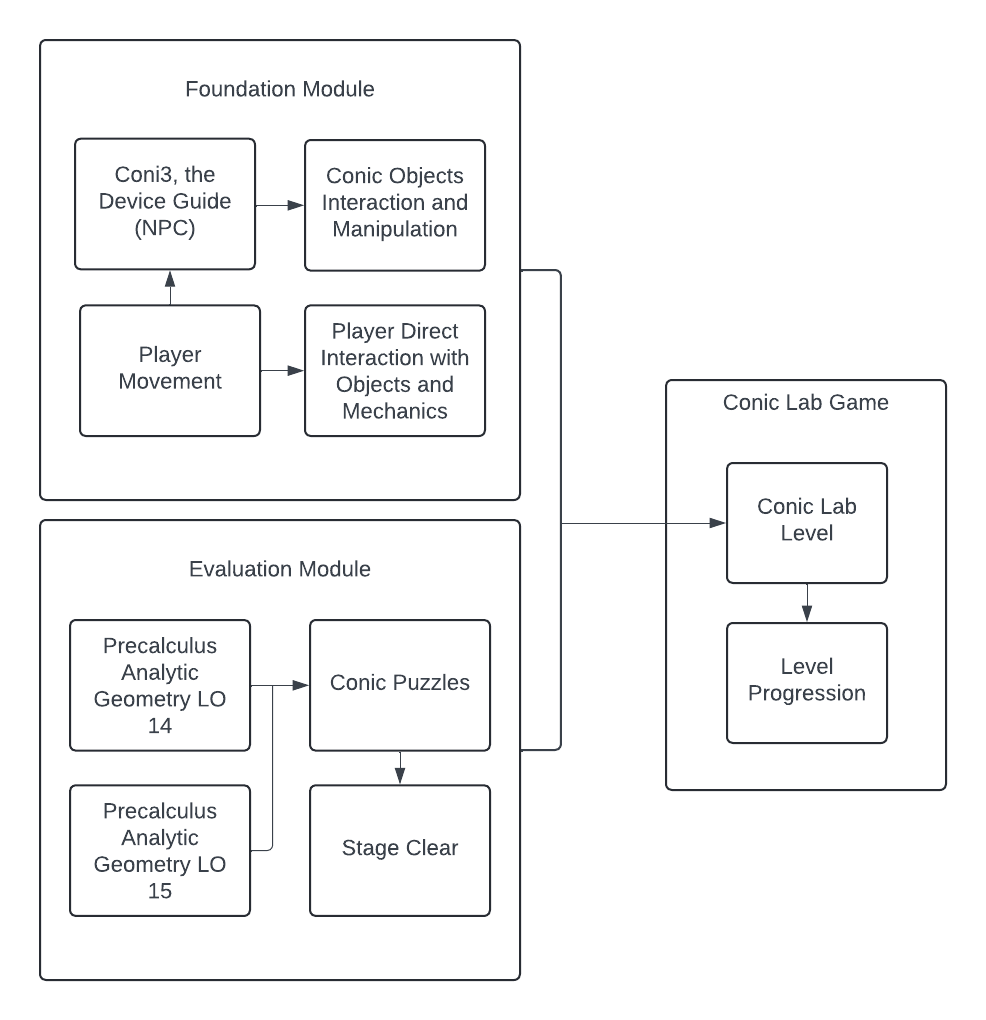
\includegraphics[width=400px,height=300px]{Chapter4/Architectural.png}      
   \caption{Architectural Design}
    \label{fig:Architectural}
\end{figure}

\subsection{Level Progression}
\label{sec:lvlprog}
Levels are divided into chapters in order to introduce each concept to the player-learner one by one. There will be a total of 4 chapters, one for each conic section: circle, ellipse, parabola, hyperbola, with 8-10 levels each to ensure the player-learner masters the concepts introduced in each chapter. Earlier levels within the chapter will be designed to be simple, only requiring minor alterations of the conic section (ex., only one variable can be altered). As the player-learner progresses to later levels in the chapter, puzzles will progressively increase in difficulty and require more alterations in the conic sections to complete the level.

\subsection{Coni3, Non-playable Character Guide and Device}
\label{sec:coni3}
The player-learner will be accompanied by a non-playable character (NPC) named Coni3 throughout the entire game. Coni3 will act as a guide and the main device with which the player-learner will interact. By interacting with the device, the respective values of H, K, A, and B can be altered to manipulate the shape of conic sections found in the level. A small guide can also be found, with the corresponding formulas and graphs for visualization for each conic section. In addition to this, Coni3 will assist player-learners when new mechanics are introduced through dialogue boxes.

\begin{figure}[H]
\hspace*{-1cm}
   \centering                  
   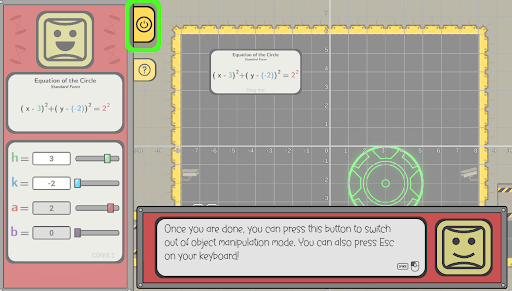
\includegraphics[width=300px,height=200px]{Chapter4/Coni3.png}      
   \caption{Meega Criteria for Game Quality Classification}
    \label{fig:MeegaCriteria}
\end{figure}

\subsection{Foundation Module}
\label{sec:foundationmodule}
This module aims to target one of the common challenges proposed by the Precalculus expert about why students were having difficulty learning Precalculus concepts. The tutorial guides the players on how to move the interactable objects and their character itself. This will help them go forward in several platform challenges within the game and they will be able to test their knowledge in conic sections through completing the game. 
These tutorials would include introducing the player to the required inputs for movement and demonstrating how to interact with game objects. New mechanics, such as linked objects, moving platforms, etc., will be introduced slowly as the player-learner progresses through the game with the assistance of the NPC guide.

\begin{figure}[H]
\hspace*{-1cm}
   \centering                  
   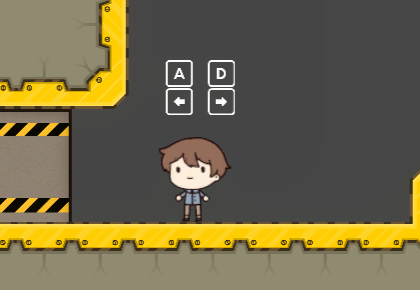
\includegraphics[width=300px,height=200px]{Chapter4/Foundation.png}      
   \caption{Player control tutorial}
    \label{fig:foundation}
\end{figure}

\subsection{Evaluation Module}
\label{sec:evaluationmodule}
For the evaluation module, there would be a series of puzzles that represent the different types of conic sections; these puzzles would be located around the level. The player is required to solve puzzles by transforming conic sections found in the level to traverse through the platforms, go through the exit gate, and complete the level. Different mechanics will be introduced throughout the game to make the levels more challenging and varied.

\begin{enumerate}
    \item \textbf{Conic Objects} - Objects resembling the conic sections are present throughout the entire game. The player learner can interact with and modify these objects using Coni3. These objects are represented by “Solid Light Constructs”, which are used as player obstructions or platforms.
\begin{figure}[H]
\hspace*{-1cm}
   \centering                  
   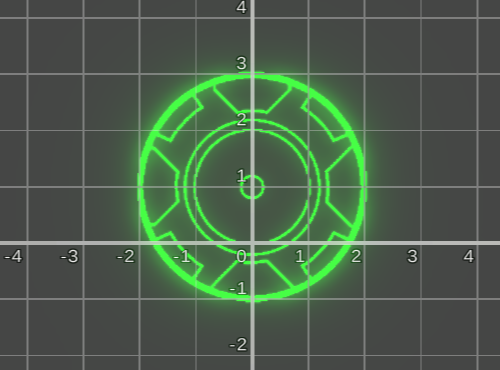
\includegraphics[width=300px,height=200px]{Chapter4/ConicObjects.png}      
   \caption{Sample of a Circle construct in the game}
    \label{fig:circleconstruct}
\end{figure}    
    \item \textbf{Key Shapes, Key Points, and Readers} - Just like Conic Objects, Key shapes may resemble one of the Conic Sections. Attached to these key shapes are key points; the key points represent the vertices (yellow) and the foci (blue) of a given conic section. The key points are then placed on to their color-matching readers. The readers act as a switch when a key point is properly placed onto it, triggering a different mechanism in the level and reversing the effect if the key point is removed.
\begin{figure}[H]
\hspace*{-1cm}
   \centering                  
   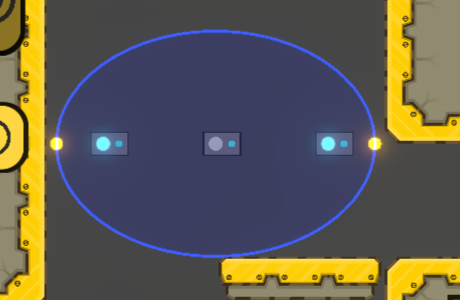
\includegraphics[width=300px,height=200px]{Chapter4/KeyShapes.png}      
   \caption{Keyshapes that requires the proper placement of foci of the ellipse }
    \label{fig:keyshapes}
\end{figure}
    \item \textbf{Pressure Plates} - Pressure plates will be activatable by the player-learner by placing weight on it, such can by placing an object on top of it or the player-learner stepping on it. Once activated, a different mechanism will be triggered at the level for the player-learner to progress (i.e., a gate opening). However, removing the weight on the pressure plate will reverse the effect it had.
\begin{figure}[H]
\hspace*{-1cm}
   \centering                  
   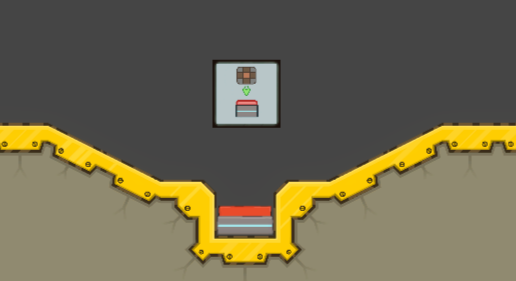
\includegraphics[width=300px,height=200px]{Chapter4/PressurePlates1.png}      
   \caption{Pressure plate with a helping instruction}
    \label{fig:pplates1}
\end{figure}
\begin{figure}[H]
\hspace*{-1cm}
   \centering                  
   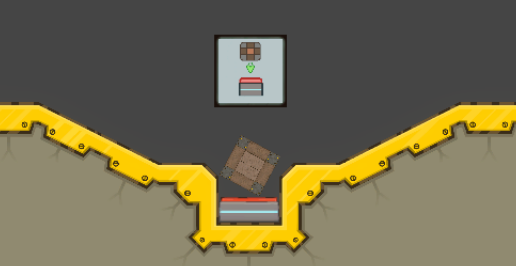
\includegraphics[width=300px,height=200px]{Chapter4/PressurePlates2.png}      
   \caption{Pressure plate being activated by applying weight to it}
    \label{fig:pplates2}
\end{figure}
    \item \textbf{Buttons} - Buttons are interactable by the player-learner and can be pressed by pressing the ‘E.’ on the keyboard. Once pressed, a different mechanism will be triggered in the level.
\begin{figure}[H]
\hspace*{-1cm}
   \centering                  
   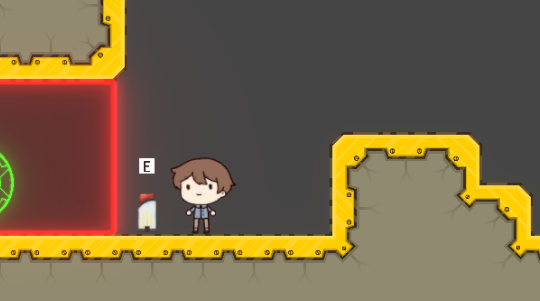
\includegraphics[width=300px,height=200px]{Chapter4/Buttons.png}      
   \caption{Players can interact with the buttons}
    \label{fig:buttons}
\end{figure}
    \item \textbf{Gates} - Gates are obstructions present within levels that the player-learner must open in order to get through.
\begin{figure}[H]
\hspace*{-1cm}
   \centering                  
   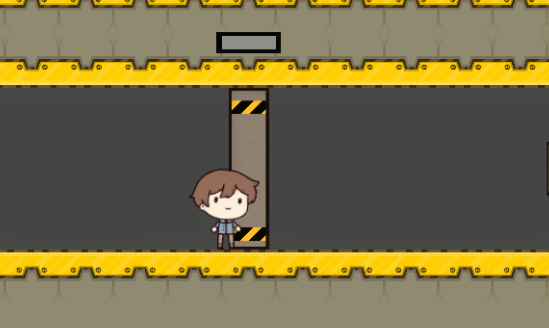
\includegraphics[width=300px,height=200px]{Chapter4/Gates.png}      
   \caption{}
    \label{fig:gates}
\end{figure}
    \item \textbf{Moving Platforms} - Moving platforms are platforms that will travel to designated points. A visual indicator will be present in order to differentiate which direction the platform will be going. The player-learner must interact with a different mechanic present within the level in order to activate the platforms.
\begin{figure}[H]
\hspace*{-1cm}
   \centering                  
   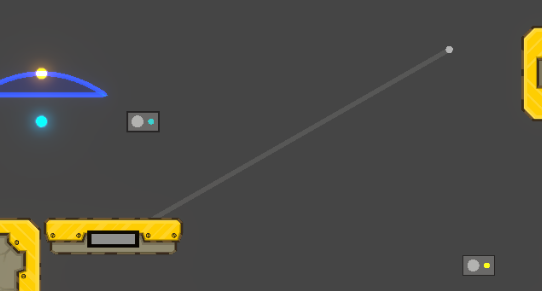
\includegraphics[width=300px,height=200px]{Chapter4/MovingPlatforms.png}      
   \caption{Moving platforms helps in crossing difficult gaps}
    \label{fig:keyshape}
\end{figure}
    \item \textbf{Disappearing Platforms} - Disappearing platforms are initially translucent, indicating that there is a possibility of making them visible. The player-learner must interact with a different mechanic present within the level in order to activate the platforms.
\begin{figure}[H]
\hspace*{-1cm}
   \centering                  
   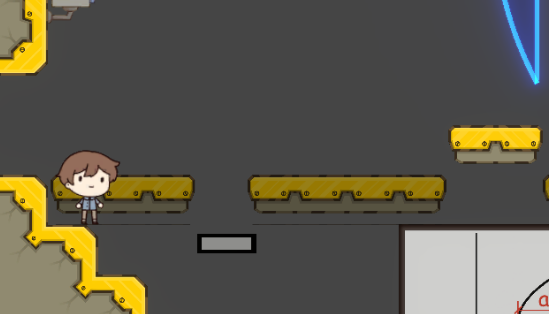
\includegraphics[width=300px,height=200px]{Chapter4/DisappearingPlatforms1.png}      
   \caption{An unactivated disappearing platform have a lighter shade than normal}
    \label{fig:dplatforms1}
\end{figure}
\begin{figure}[H]
\hspace*{-1cm}
   \centering                  
   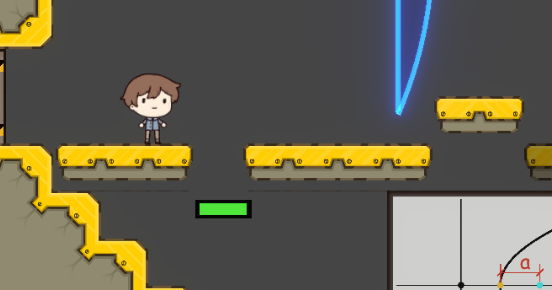
\includegraphics[width=300px,height=200px]{Chapter4/DisappearingPlatforms2.png}      
   \caption{When the proper mechanics get activated, it makes the platform appear}
    \label{fig:dplatforms2}
\end{figure}
    \item \textbf{Linked Objects} - Linked objects are objects that can be altered by the player-learner. The movement of one object causes the other object linked to it to move as well.
\begin{figure}[H]
\hspace*{-1cm}
   \centering                  
   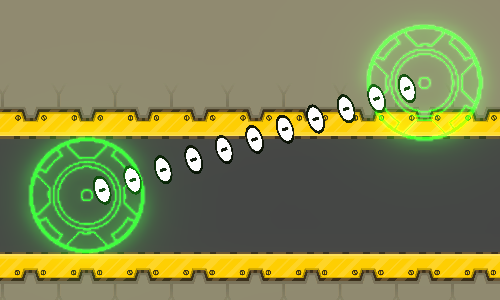
\includegraphics[width=300px,height=200px]{Chapter4/LinkedObjects.png}      
   \caption{A chain between constructs indicate that they are linked objects}
    \label{fig:linkedobjects}
\end{figure}
\end{enumerate}


\subsection{Software Functions}
The software functions of the GBLE are the following:

\begin{enumerate}
    \item \textbf{Main Menu} - The main menu is the screen that will be displayed to the player when the application is launched. Here, all the levels are displayed, and information on which levels have been completed is also contained.
    \item \textbf{Pause} - Inside each level, there will be a pause button in the upper right corner. Clicking on this opens a new interface with two possible selections: resume and level select.
    \item \textbf{Resume} - This is a button found when the pause button is clicked. Pressing this button simply returns the player back to the game screen.
    \item \textbf{Level Select} - This button is found when pressing the pause button. Clicking this button will return the player to the main menu.
    \item \textbf{Retry} - Similar to the pause button, the retry button is found on each level and is just beside the pause button in the upper right corner. This button simply restarts the level, moving the player back to the spawn point.
    \item \textbf{Device} - The device is found on the left side of the screen at each level. It is where the player is able to change the values of H,K, A, and b of each conic shape. 
    \item \textbf{Help} - This is the button found beside the device with a question mark symbol in it. Clicking on this allows the player to open a guide consisting of the formulas of each of the conic shapes and some other tips that could help deal with the different mechanics inside the game.
    \item \textbf{Back} - This is the button found beside the device above the help button with a power symbol. Pressing this button returns the player to the game screen.
    \item \textbf{Shape Interaction} - Clicking on a conic object “turns on” the device, allowing the player to manipulate the variables of the shape. When a conic object is clicked, the grid view is shown to the player, and the cartesian plane is overlaid onto the level to assist the players in determining where the shapes are located.
\end{enumerate}

\section{Physical Environment and Resources}
The GBLE was developed using Unity as its game engine, and was designed for desktop computers, and is able to be run even with a “low-end” PC. Inputs will only be accepted through the mouse and keyboard connected to the PC.



%%%%%%%%%%%%%%%%%%%%%%%%%%%%%%%%%%%%%%%%%%%%%%%%%%%%%%%%%%%%%%%%%%%%%%%%%%%%%%%%%%%%%%%%%%%%%%%%%%%%%%
%
%   Filename    : abstract.tex 
%
%   Description : This file will contain your abstract.
%                 
%%%%%%%%%%%%%%%%%%%%%%%%%%%%%%%%%%%%%%%%%%%%%%%%%%%%%%%%%%%%%%%%%%%%%%%%%%%%%%%%%%%%%%%%%%%%%%%%%%%%%%

\chapter{Design and Implementation Issues}
\label{sec:designAndImplementation}

\section{Conic Object Readability and Recognition}
Initially, conic objects resembled objects that existed within the world space. However, a concern arose that the players might not realize that conic objects can be positioned within terrain or go through "solid" objects that the player would not be able to go through. To make it clear that conic objects are able to have said behavior, the sprites used were changed to resemble "light constructs" and added a level that demonstrates that the objects could move through terrain.
\section{Conic Equation Signposting}
During the game's initial testing, a concern arose: During gameplay, testers barely noticed or looked at the equation of the object they were manipulating; this is caused by the equation's position on the screen being above the UI controls, where testers would look at the object being manipulated and then to the UI controls and back to the object without taking a look at the equation. To make the object's equation more apparent and noticeable, a floating text box containing the equation was added. The text box's position was dependent on where the object being manipulate was located as to not block vision of the object.
\section{Level Order and Progression}
Initially, the levels were ordered by their complexity to complete, with no regard to the focused conic type of the level. This type of ordering could lead to players being overwhelmed with the number of new concepts being introduced by each shape. The levels were now reordered into sections, where each section focused on a conic shape. The current order is as follows: Circles $>$ Ellipses $>$ Parabolas $>$ Hyperbolas. Ordering by complexity was still followed within these sections. 
%%%%%%%%%%%%%%%%%%%%%%%%%%%%%%%%%%%%%%%%%%%%%%%%%%%%%%%%%%%%%%%%%%%%%%%%%%%%%%%%%%%%%%%%%%%%%%%%%%%%%%
%
%   Filename    : abstract.tex 
%
%   Description : This file will contain your abstract.
%                 
%%%%%%%%%%%%%%%%%%%%%%%%%%%%%%%%%%%%%%%%%%%%%%%%%%%%%%%%%%%%%%%%%%%%%%%%%%%%%%%%%%%%%%%%%%%%%%%%%%%%%%

\chapter{Results and Discussion}
\label{sec:results }

\section{Results Overview}
\label{sec:resultoverview}
In this chapter, the data gathered from the pre-tests, game test, and post-tests are gathered in order to see the effect of Conic Lab in helping player-learners perform better on Precalculus Conic Sections. 

%%%%%%%%%%%%%%%%%%%%%%%%%%%%%%%%%%%%%%%%%%%%%%%%%%%%%%%%%%%%%%%%%%%%%%%%%%%%%%%%%%%%%%%%%%%%%%%%%%%%%%
\begin{comment}
% Conic Lab Pre-test and Post Test
A pre-test was given to the participants before they were allowed to test the game. This was done in order to determine the participant's baseline knowledge about the topic of Precalculus conic sections. There were a total of 12 participants, which are all senior high school students from STEM strand and had a prior experience with learning about the target Precalculus topic for the game. These students range from grade 11 and grade 12. The participants were asked to take the pre-test before testing the game, which would be followed by a post-test after in order to compare their two scores with each other.

The conic test was divided to the four types of conic sections: circle, parabola, ellipse, and hyperbola. The goal is to determine their level of understanding for each of them. Each type of the conic sections have multiple problems about them with varying difficulty.

% MEEGA / Player Opinion
% - Notable trend on the player opinion survey
% Behavioral Analysis 
% - Notable behavior of the participants
% No need for performance testing
\end{comment}
%%%%%%%%%%%%%%%%%%%%%%%%%%%%%%%%%%%%%%%%%%%%%%%%%%%%%%%%%%%%%%%%%%%%%%%%%%%%%%%%%%%%%%%%%%%%%%%%%%%%%%
\subsection{Pre-test and Post-test Results}
Before performing the statistical analysis on the pre-test and post-test data, a test of Normality, the Shapiro-Wilk test, is performed to check the Normality of the data by the difference between the pre-test and post-test with an $\alpha$ = 0.05. The Normality test is done due to the number of participants n = 14. Test results show a p-value = 0.24 $>$ $\alpha$ = 0.05, showing that the data has no significant departure from normality, and we can proceed with a parametric test, a Paired T-Test.

\begin{table}[h]
	\centering
	\caption{Test of Normality (Shapiro-Wilk)}
	\label{tab:testOfNormality(Shapiro-Wilk)}
	{
		\begin{tabular}{lrrrr}
			\toprule
			 &  &  & W & p  \\
			\cmidrule[0.4pt]{1-5}
			Pre-test & - & Post-test & $0.919$ & $0.240$  \\
			\bottomrule
			% \addlinespace[1ex]
			% \multicolumn{5}{p{0.5\linewidth}}{\textit{Note.} Significant results suggest a deviation from normality.} \\
		\end{tabular}
	}
\end{table}

For this study the following are the null hypothesis and the alternative hypothesis:


\begin{tabular}{p{13cm} @{\hspace{1cm}} p{12cm}} 
\textbf{H0:}There is no significant difference between the mean scores of the pre-test and post-test \\ \\
\textbf{H1:}There is significant difference between the mean scores of the pre-test and post-test
\end{tabular}

Given the null and alternative hypotheses, to assess if there was a significant change between the participants’ pre-test and post-test scores, a One-Tailed Paired T-test and a Wilcoxon Signed-Rank test were performed on the data using $\alpha$ = 0.05. Table~\ref{tab:pairedSamplesT-Test} presents the summarized results for the Paired T-Test and Wilcoxon Signed-Rank Test. 



\begin{table}[h]
	\centering
	\caption{Paired Samples T-Test \& Wilcoxon Signed-Rank Test Results}
	\label{tab:pairedSamplesT-Test}
	{
		\begin{tabular}{lrrrrrrr}
			\toprule
			Measure 1 &  & Measure 2 & Test & Statistic & z & df & p  \\
			\cmidrule[0.4pt]{1-8}
			Pre-test & - & Post-test & Student & $-4.189$ & $$ & $12$ & .00063  \\
			$$ & $$ & $$ & Wilcoxon & $0.000$ & $-2.934$ & $$ & $0.002$  \\
			\bottomrule
			% \addlinespace[1ex]
			% \multicolumn{8}{p{0.5\linewidth}}{\textit{Note.} For all tests, the alternative hypothesis specifies that Pretest is less than Posttest.} \\
		\end{tabular}
	}
\end{table}
As shown in table~\ref{tab:pairedSamplesT-Test}, the T-Test's p-value = 0.00063 is less than $\alpha$ = 0.05, suggesting that the difference between the pre-test and post-scores is significant. To further support the t-test observation, the Wilcoxon Signed-Rank test shows a W Statistic of 0, and with $\alpha$ = 0.05 and a sample size of 11 as those whose scores had no difference for both tests were not included, the Critical Value is 10. With the W = 0 $<$ Critical Value = 10, and the shown p-value = 0.002 $<$  $\alpha$ = 0.05, this test also suggests a significant difference in scores between the pre-test and post-test. With the results of both tests, there is substantial evidence to reject the null hylpothesis and say that there is a change in participants' scores after playing the game.

\iffalse
\clearpage
\begin{table}[h]
\hspace*{-1cm}
\begin{tabular}{|c|c|c|c|c|c|c|c|c|}
\hline
$n$ & Pretest & Posttest & Difference & Sign & Absolute Difference & Rank & Rank - & Rank + \\
\hline
1 & 5.00 & 6.00 & -1.00 & -1 & 1 & 1 & 1 & \\
2 & 12.00 & 14.00 & -2.00 & -1 & 2 & 3 & 3 & \\
3 & 7.00 & 13.00 & -6.00 & -1 & 6 & 8.5 & 8.5 & \\
4 & 9.00 & 13.00 & -4.00 & -1 & 4 & 6.5 & 6.5 & \\
5 & 7.00 & 13.00 & -6.00 & -1 & 6 & 8.5 & 8.5 & \\
6 & 9.00 & 9.00 & 0.00 & 0 & - & - & & \\
7 & 5.00 & 7.00 & -2.00 & -1 & 2 & 3 & 3& \\
8 & 2.00 & 2.00 & 0.00 & 0 & - & - & & \\
9 & 11.00 & 13.00 & -2.00 & -1 & 2 & 3 & 3 & \\
10 & 10.00 & 13.00 & -3.00 & -1 & 3 & 5 & 5 & \\
11 & 4.00 & 12.00 & -8.00 & -1 & 8 & 10 & 10 & \\
12 & 6.00 & 10.00 & -4.00 & -1 & 4 & 6.5 & 6.5 & \\
13 & 3.00 & 14.00 & -11.00 & -1 & 11 & 11 & 11 & \\
\hline
 & & & & & & Total & 66(W-) & 0(W+) \\
\hline
\end{tabular}
\caption{Full Wilcoxon Signed-Rank Test}
\label{tab:pretest_posttest_comparison}
\end{table}
\fi


\subsection{MEEGA+ Results}
Particiants' responses for the MEEGA survey are represented as follows.

\begin{center}

\begin{tabular}{|c|c|}
\hline
\textbf{Response} & \textbf{Value} \\
\hline
Strongly Agree & 2 \\
\hline
Agree & 1 \\
\hline
Neutral & 0 \\
\hline
Disagree & -1 \\
\hline
Strongly Disagree & -2 \\
\hline
\end{tabular}
\captionof{table}{Response Values Table}
\end{center}

The averaged scores for the ratings of the participants for each quality factor are positive. The higher scoring quality factors include the games design and the pacing of new challenges both scoring 1.84, the games ability to provide a satisfying feeling of accomplishment with a score of 1.76, and how fun the player had with a score of 1.69. On the other hand, the lower scoring quality factors include, the level of immersion/engagement the player had scoring 0.92, how relevant the game content is to the players interests with 0.84, and the players preference to use the game to learn the material scoring 0.53. \\

To classify the game's quality level, the participants responses are use and to be compared to the criteria as shown in Figure~\ref{fig:MeegaCriteria}. The average of all scores is computed as $\theta$=1.27. $\theta$ is then transformed by a scale of (50,15) with the formula $\theta_{50,15}=50+15* \theta_{1.27}$ resulting in a value of 69.15. This value classifies our game as excellent quality given that $\theta >=$ 65.

\begin{figure}[h]
\hspace*{-1cm}
   \centering                  
   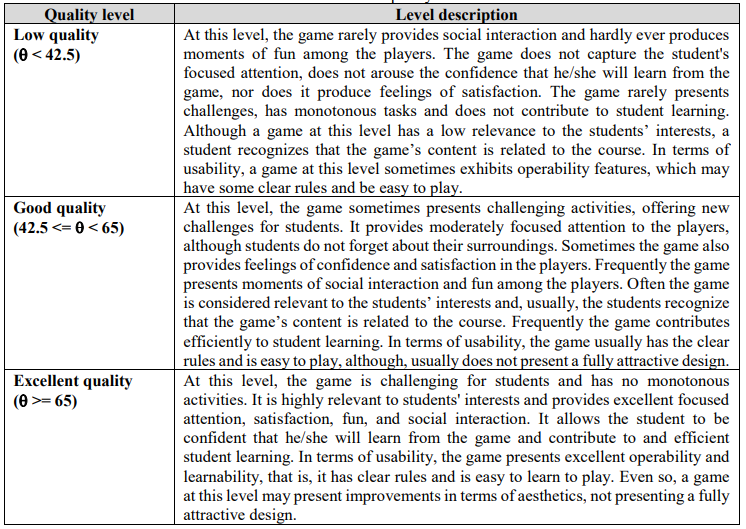
\includegraphics[width=300px,height=200px]{Chapter6/MeegaCriteria.png}      
   \caption{Meega Criteria for Game Quality Classification}
    \label{fig:MeegaCriteria}
\end{figure}
\section{Discussion}

\subsection{Pre-Test and Post-Test Data}
The statistical analysis showed a significant improvement in participants' scores from the pre-test to the post-test, suggesting the game's effectiveness in teaching/improving the participant's understanding of the conic sections. Pre-test scores showed no noticeable patterns in which questions were answered correctly. However, post-test scores indicated a higher likelihood of participants answering correctly in questions involving circles and parabolas and less so for questions involving ellipses and hyperbolas. In terms of improvement, participants improved the most in answering questions that asked them to identify the equation of the conic given specific details of the shape or vice versa.


\subsection{Meega+ Discussion}
Based on the MEEGA results, there were several factors of the game that were positively evaluated by the participants. Specifically, these aspects have scored notably high: game design, pacing of challenges, and overall fun factor. These elements are crucial as they directly contribute to player enjoyment and satisfaction. On the other hand, there were also low scores on some aspects. Specifically, these are the immersion/engagement, relevance to player interests, and educational value aspects.

The game is categorized as "excellent" by the computed average score. This ranking emphasizes the game's capacity to provide enjoyable gameplay and an immersive experience. There is room for development, nevertheless, as evidenced by the lower ratings for immersion, relevance to player interests, and instructional value. In order to improve player engagement and better match the game with player preferences and educational goals, future versions may concentrate on improving these features. The game can be made even better and more efficient by taking care of these issues.



 
%%%%%%%%%%%%%%%%%%%%%%%%%%%%%%%%%%%%%%%%%%%%%%%%%%%%%%%%%%%%%%%%%%%%%%%%%%%%%%%%%%%%%%%%%%%%%%%%%%%%%%
%
%   Filename    : abstract.tex 
%
%   Description : This file will contain your abstract.
%                 
%%%%%%%%%%%%%%%%%%%%%%%%%%%%%%%%%%%%%%%%%%%%%%%%%%%%%%%%%%%%%%%%%%%%%%%%%%%%%%%%%%%%%%%%%%%%%%%%%%%%%%

\chapter{Conclusion}
\label{sec:results }

\section{Conclusion}
Two learning outcomes (LOs) were selected from the Analytical Geometry content found in the Department of Education’s curriculum guide for Senior High School STEM Course, as the target learning outcomes. Concepts regarding conic sections were focused on, specifically recognizing equations and important characteristics of different  of conic sections and solving situations involving conic sections.

Given these target learning outcomes, LO mechanics were designed to be used as game mechanics. These LO mechanics were integrated, playtested, and evaluated periodically, with alterations depending on whether the LO was achieved, and to what extent. Puzzles mechanics, levels, and other interactable mechanics were developed to target specific concepts related to the LOs, with each mechanic relevant in the level's solution, ensuring the player-learner's mastery in each concept.

A GBLE with the purpose as an assistive tool to achieving the selected learning outcomes was developed in the Unity game engine, with LO mechanics as a part of the core gameplay loop and several non-LO mechanics to support it. Additionally, gamification elements such as narrative, objectives, level progression and challenges were included in the GBLE to enhance the engagement and motivation of player-learners.

A pre-test and post-test comparison and a MEEGA+ survey were conducted to evaluate the GBLE's effects on supporting the achievement of the target LOs as well as the engagement of the player-learners. In order to compare the pre-test and post-test results, a paired t-test and a Wilcoxon signed-rank test were performed to gauge the GBLE's effectiveness in the support of the achievement of the target LOs.

The study results suggest that the game-based learning environment significantly supports the achievement of the selected target LOs of the player-learners, while keeping them engaged. The pre-test and post-test comparison results show that there is a significant difference after playtesting, with higher scores on the post-test. While some factors in the MEEGA+ survey received low scores, the average scores of all factors still classify the game's quality as excellent.

\section{Recommendations}
\label{sec:recommendations}
One of the things that Conic Lab could have improved on was achieving another gamification method for the players through the use of an achievement system. For example, when a player completes a level in the least moves possible, then they could receive a green highlight for the level in the main menu. This could improve the engagement/immersion of the players as they will receive a reward which would also signify that they were efficient in a level. 

The amount of playtesting could be improved to generate more ideas as to where the game could be more refined. In one group of playtesters, a lot of information and point for improvements have already been discovered such as adding music, improving the immersive experience when playing the game, and so on. More playtesting would allow Conic Lab to discover more areas to improve on and this could make the game better.

Lastly, a mobile phone version for the game would also be helpful. It would allow more room for students to play the game as more people have phones rather than personal computers. Accessibility would also be improved and this could lead to more playtesters.

Added Chapter 7





 

\appendix                         %-- used to specify appendices
%%%%%%%%%%%%%%%%%%%%%%%%%%%%%%%%%%%%%%%%%%%%%%%%%%%%%%%%%%%%%%%%%%%%%%%%%%%%%%%%%%%%%%%%%%%%%%%%%%%%%%
%
%   Filename    : appendix_A.tex 
%
%   Description : This file is one of the appendices. 
%                 
%%%%%%%%%%%%%%%%%%%%%%%%%%%%%%%%%%%%%%%%%%%%%%%%%%%%%%%%%%%%%%%%%%%%%%%%%%%%%%%%%%%%%%%%%%%%%%%%%%%%%%

\chapter{Ethics Forms}
\label{sec:appendixa}


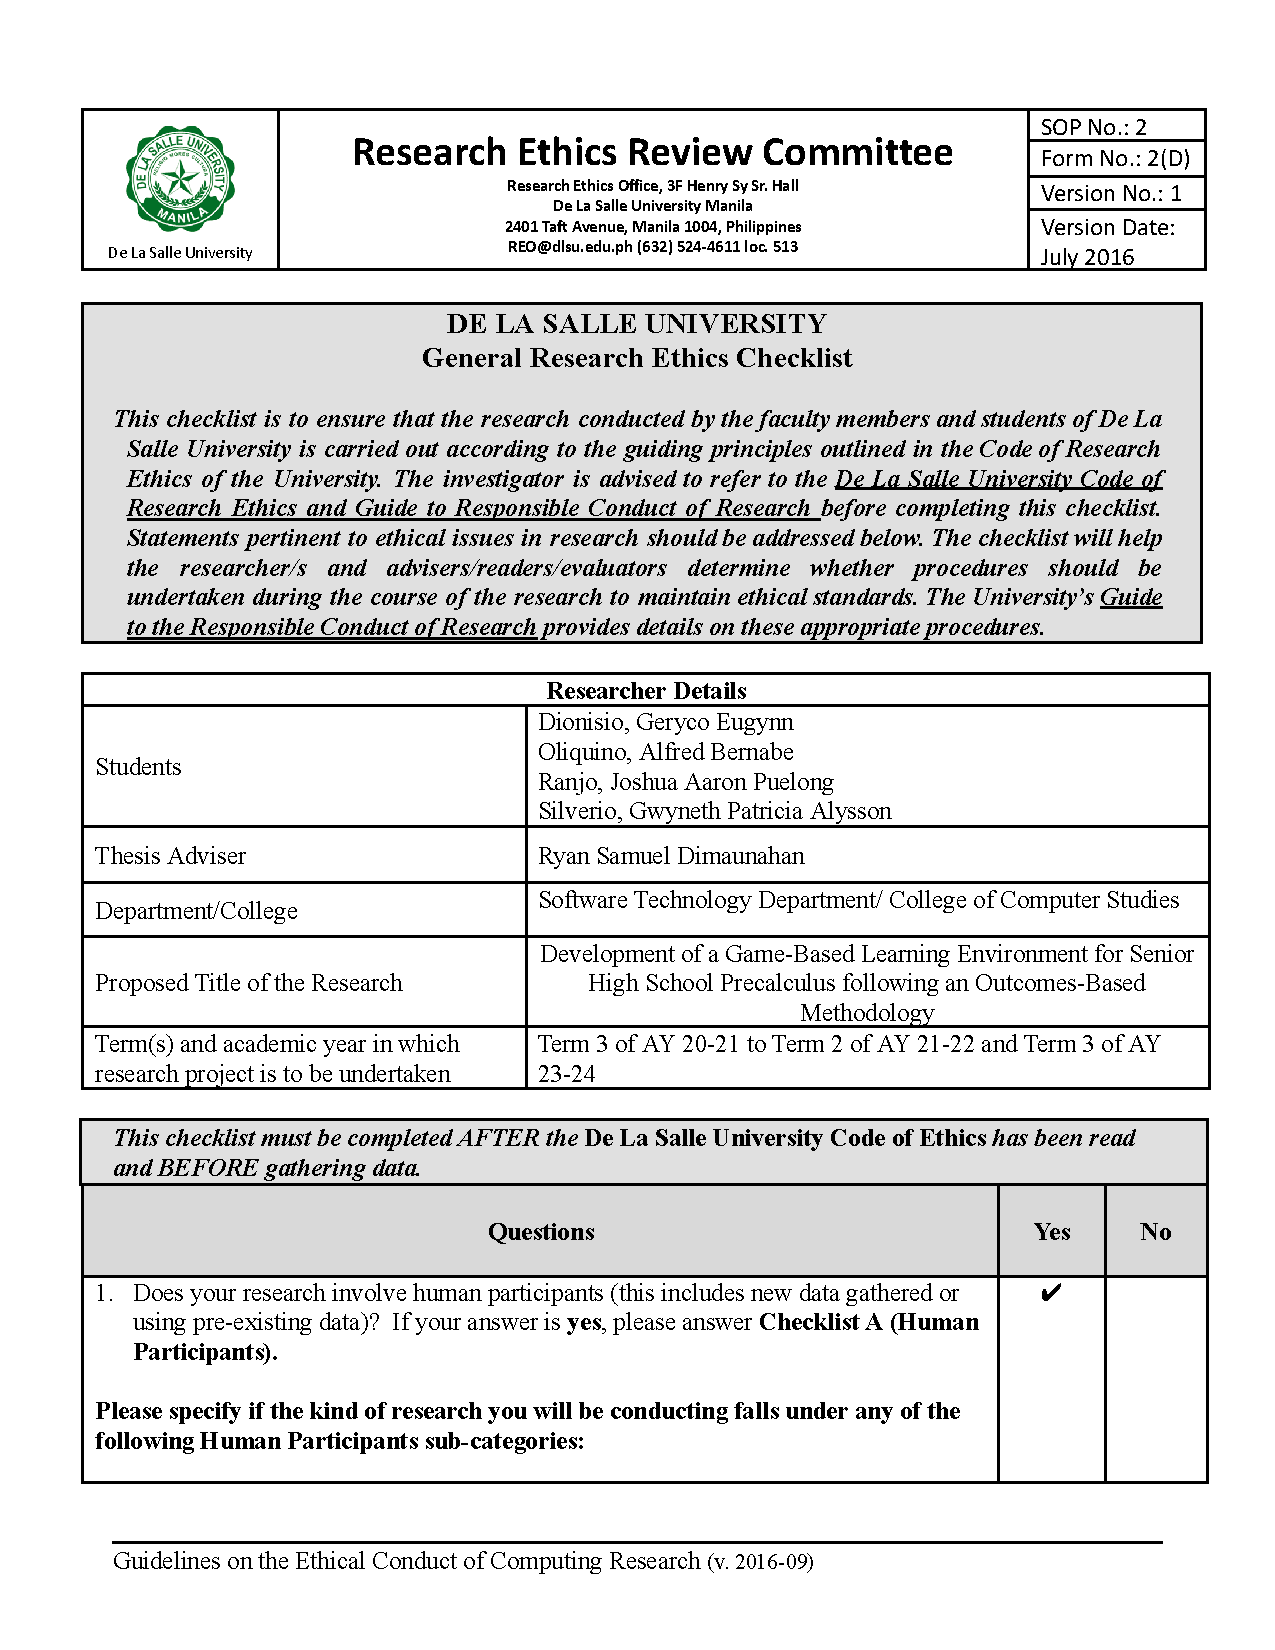
\includepdf[scale=0.9, pages=-, offset=-1.2cm 0cm]{Appendices/General-Research-Ethics-Checklist.pdf}

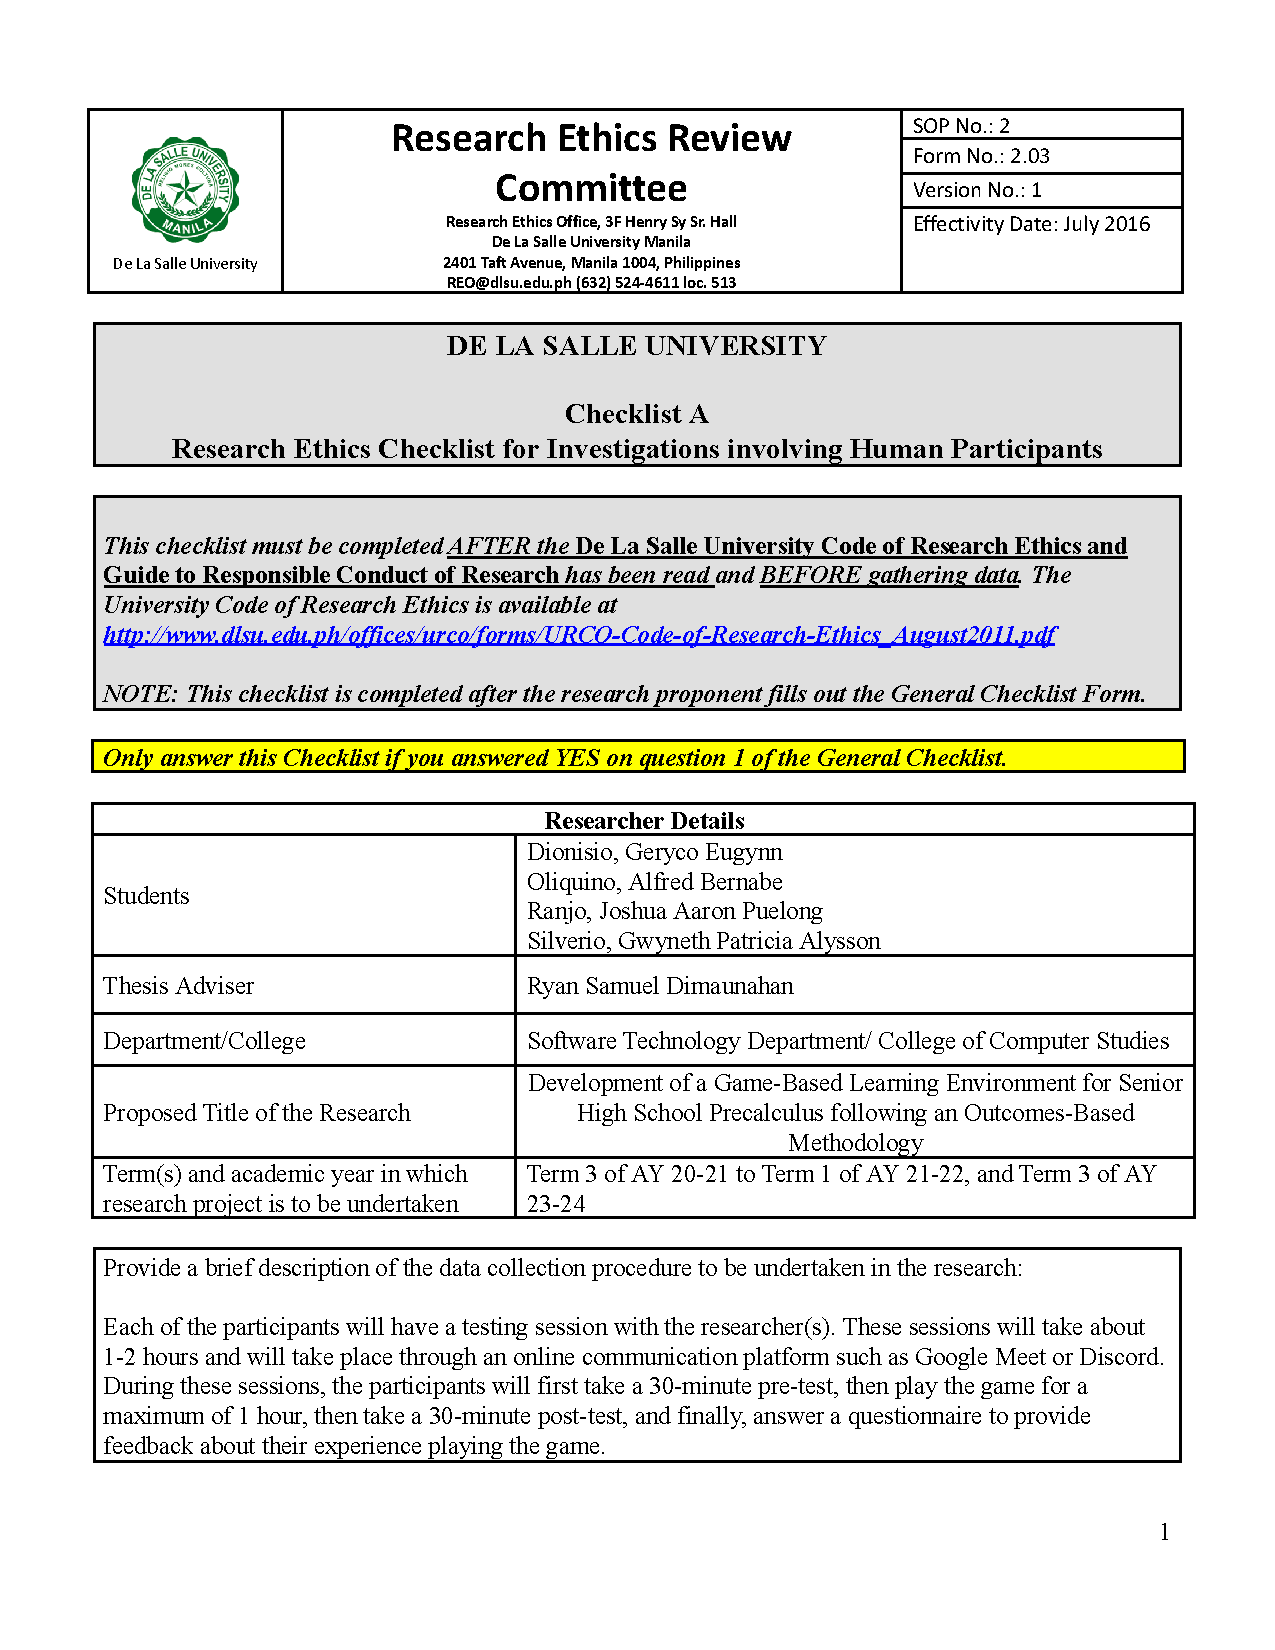
\includepdf[scale=0.9, pages=-, offset=-1.2cm 0cm]{Appendices/ChecklistA-HumanParticipants.pdf}

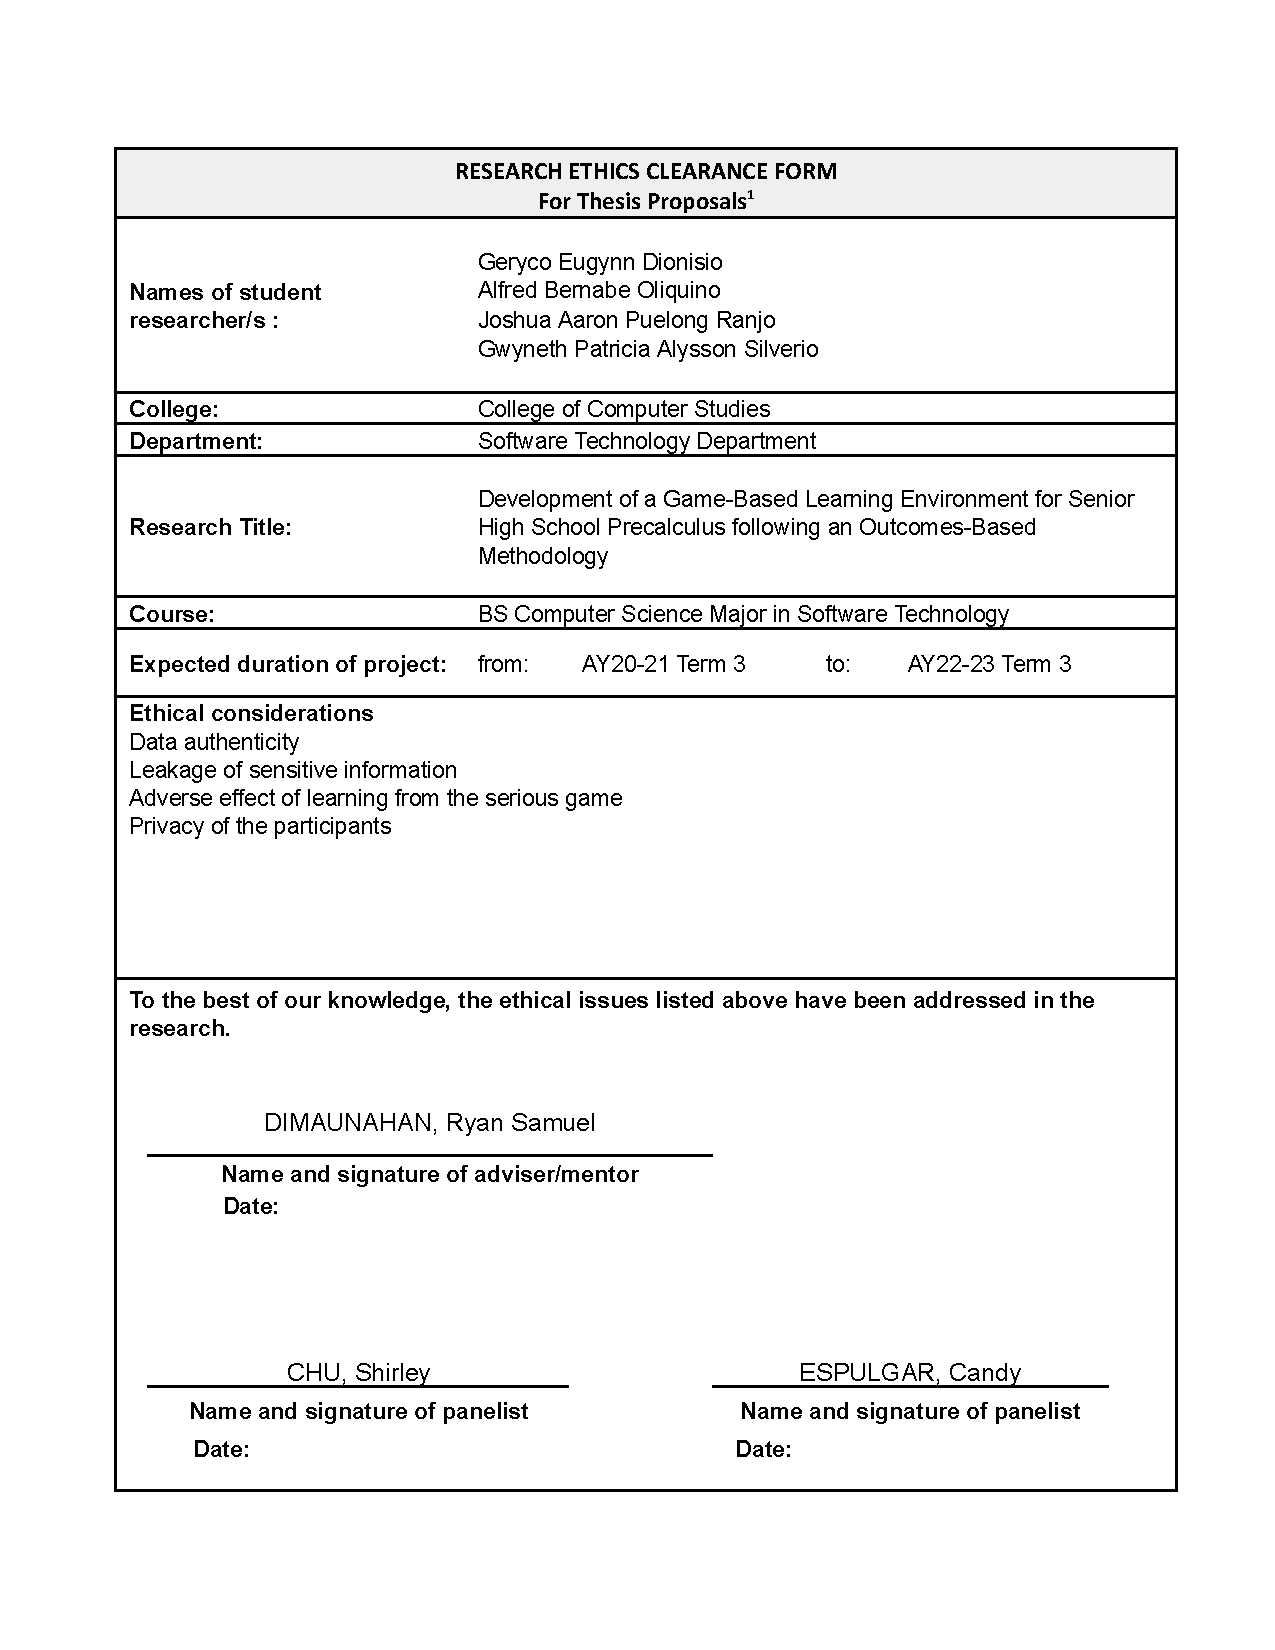
\includepdf[scale=0.9, pages=-, offset=-1.2cm 0cm]{Appendices/Research-Ethics-Clearance-Form.pdf}

              %-- includes LaTeX source file for Appendix A
                                                 %-- your job: **CREATE/EDIT** your own source file for the appendices

%%%%%%%%%%%%%%%%%%%%%%%%%%%%%%%%%%%%%%%%%%%%%%%%%%%%%%%%%%%%%%%%%%%%%%%%%%%%%%%%%%%%%%%%%%%%%%%%%%%%%%
%
%   Filename: appendix_B.tex 
%
%   Description : This file will contain one of your appendices.
%                 
%%%%%%%%%%%%%%%%%%%%%%%%%%%%%%%%%%%%%%%%%%%%%%%%%%%%%%%%%%%%%%%%%%%%%%%%%%%%%%%%%%%%%%%%%%%%%%%%%%%%%%

\chapter{Turnitin}
\label{sec:appendixb}

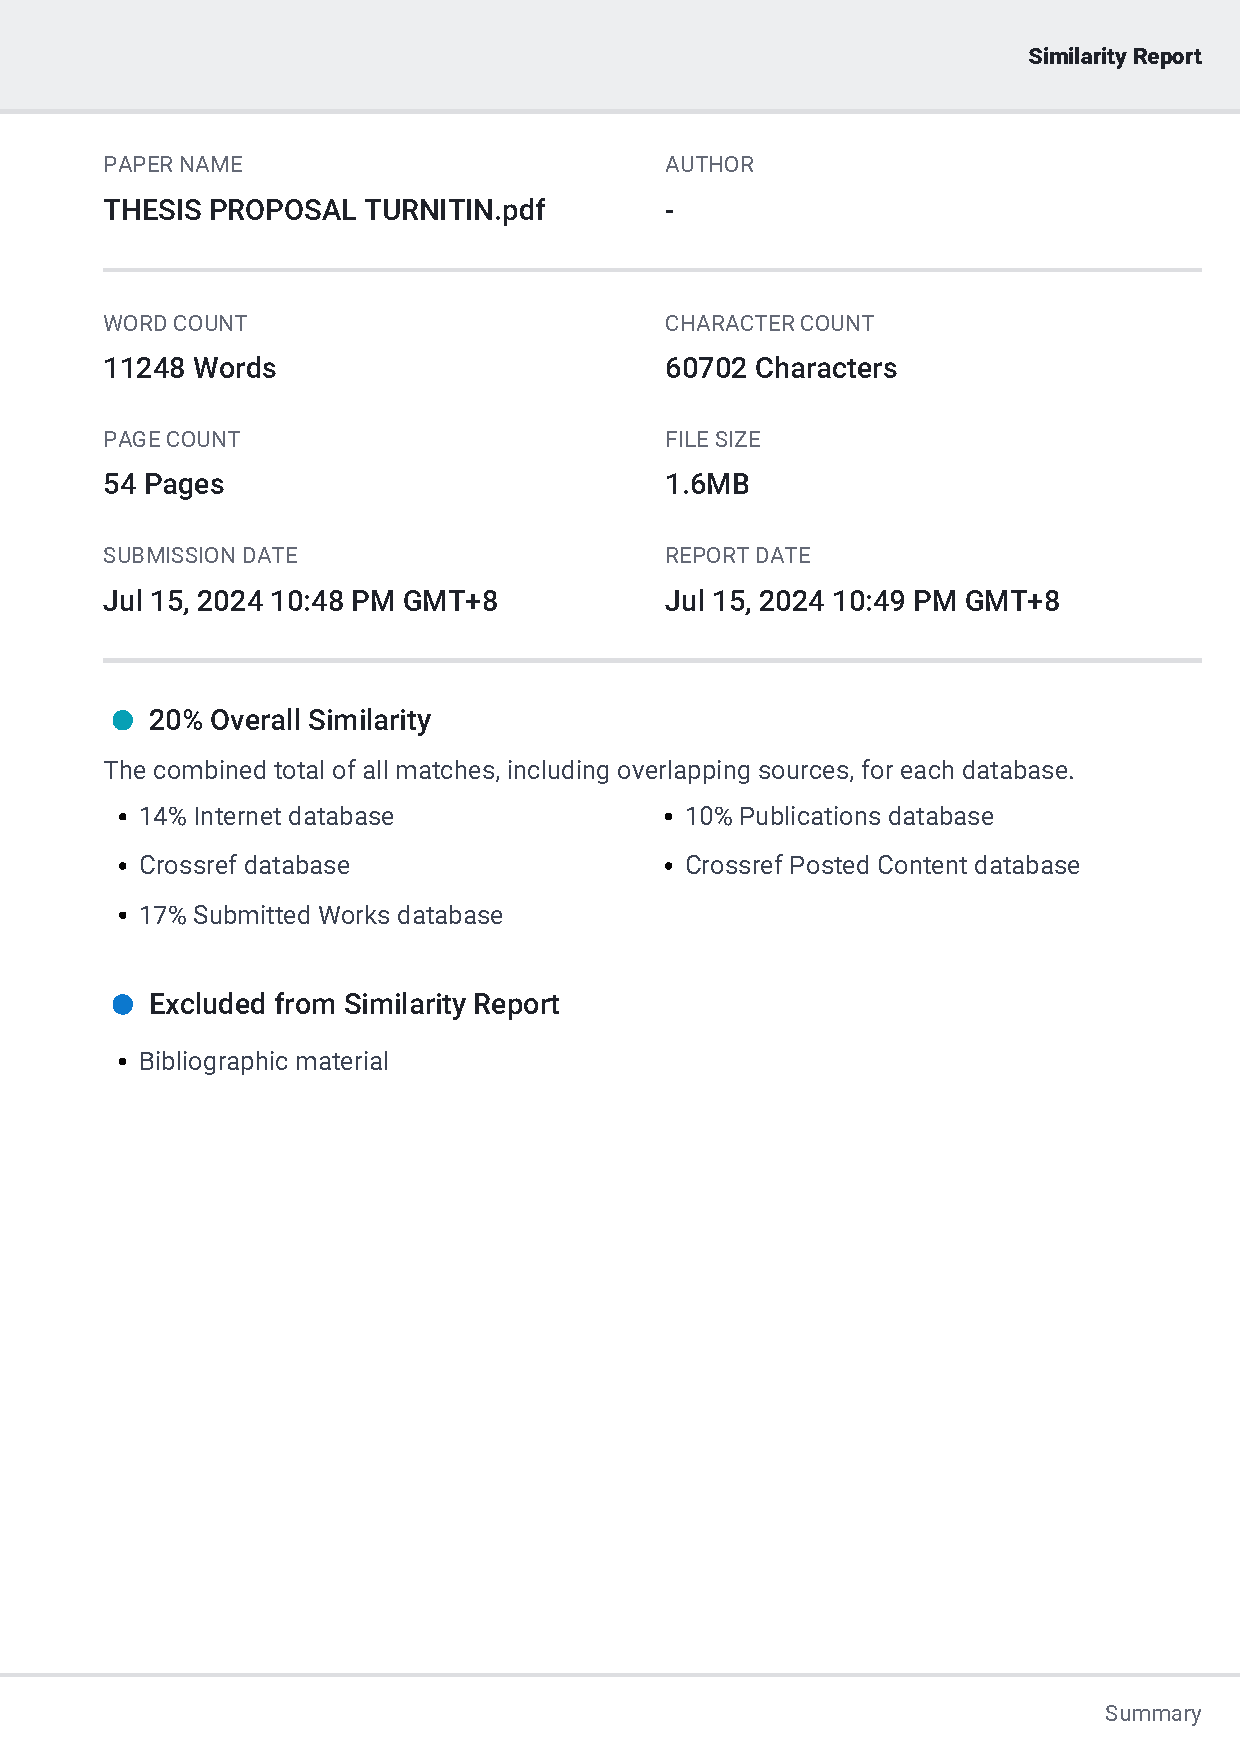
\includepdf[scale=0.9, pages=-, offset=-1.2cm 0cm]{Appendices/Turnitin-Result.pdf}

%%%%%%%%%%%%%%%%%%%%%%%%%%%%%%%%%%%%%%%%%%%%%%%%%%%%%%%%%%%%%%%%%%%%%%%%%%%%%%%%%%%%%%%%%%%%%%%%%%%%%%
%
%   Filename    : appendix_C.tex
%
%   Description : This file will contain information about your Resource Persons
%                 
%%%%%%%%%%%%%%%%%%%%%%%%%%%%%%%%%%%%%%%%%%%%%%%%%%%%%%%%%%%%%%%%%%%%%%%%%%%%%%%%%%%%%%%%%%%%%%%%%%%%%%

\chapter{Resource Persons}
\label{sec:appendixc}

%
%  Indicate your resource persons here:
%
%	<full name and title, e.g., Dr. Juan de la Cruz>
%	<profession, e.g., faculty>
%	<department, e.g., College of Computer Studies>
%	<name of institution, e.g., De La Salle University>
%	<e-mail address>
%
%

%
%  the following shows 3 examples, replace entries with your own
%
\newcommand{\resperson}[4]{\textbf{#1} \\ #2 \\ #3 \\ \url{#4}\vspace{0.5em}\\}

\resperson{Geryco Eugynn Dionisio}{Researcher}{College of Computer Studies}{geryco_dionisio@dlsu.edu.ph}
\resperson{Alfred B. Oliquino}{Researcher}{College of Computer Studies}{alfred_oliquino@dlsu.edu.ph}
\resperson{Joshua Aaron P. Ranjo}{Researcher}{College of Computer Studies}{joshua_ranjo@dlsu.edu.ph}
\resperson{Gwyneth Patricia Alysson P. Silverio}{Researcher}{College of Computer Studies}{gwyneth_silverio@dlsu.edu.ph}
\resperson{Mr. Ryan Samuel Dimaunahan}{Adviser}{College of Computer Studies\\De La Salle University-Manila}{ryan.dimaunahan@dlsu.edu.ph}

%%%%%%%%%%%%%%%%%%%%%%%%%%%%%%%%%%%%%%%%%%%%%%%%%%%%%%%%%%%%%%%%%%%%%%%%%%%%%%%%%%%%%%%%%%%%%%%%%%%%%%
%
%   Filename: appendix_D.tex 
%
%   Description : This file will contain one of your appendices.
%                 
%%%%%%%%%%%%%%%%%%%%%%%%%%%%%%%%%%%%%%%%%%%%%%%%%%%%%%%%%%%%%%%%%%%%%%%%%%%%%%%%%%%%%%%%%%%%%%%%%%%%%%

\chapter{Meega+ Questionnaire}
\label{sec:appendixd}

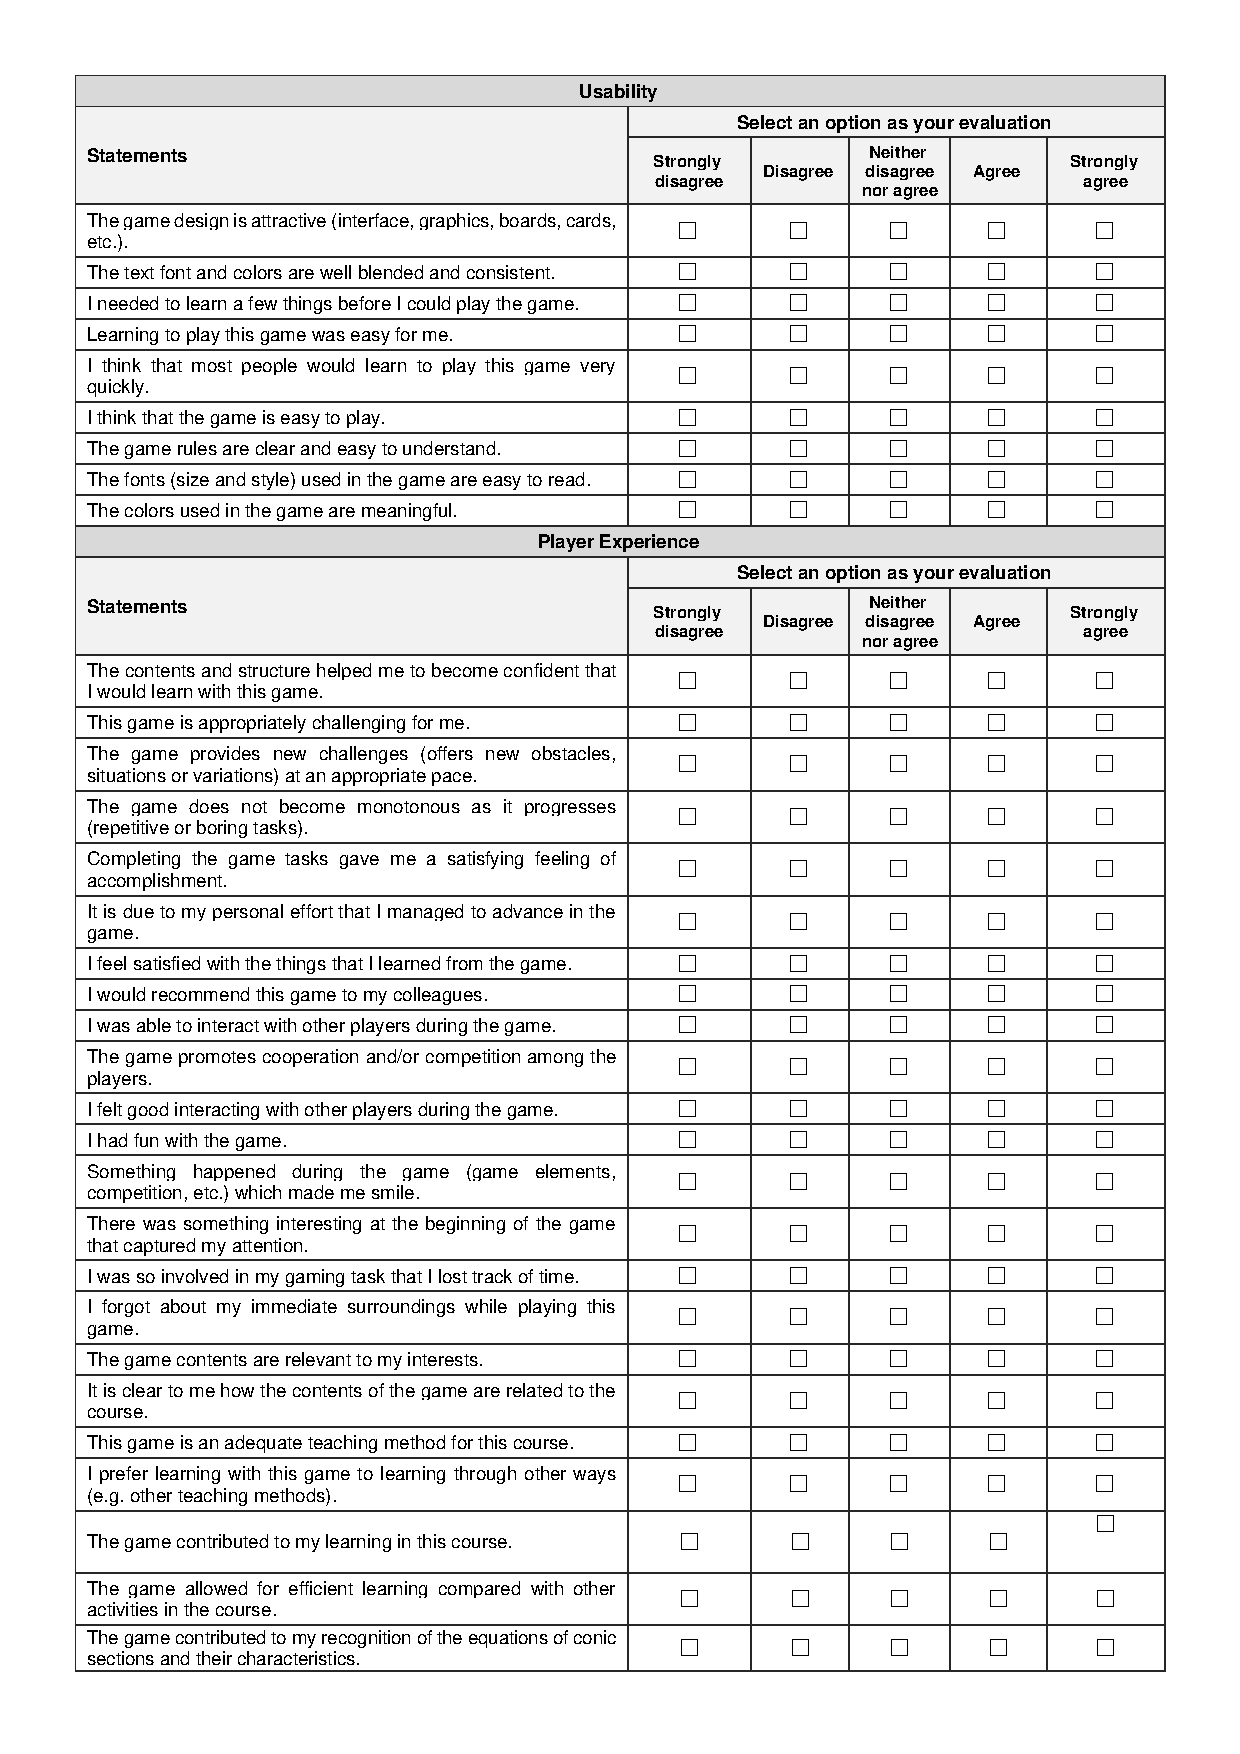
\includepdf[pages=-,offset=-1.5cm 0cm]{Appendices/MeegaQuestionnaire.pdf}

\chapter{Meega+ Analysis}
\label{sec:appendixe}
\newpage
\hspace{1cm}
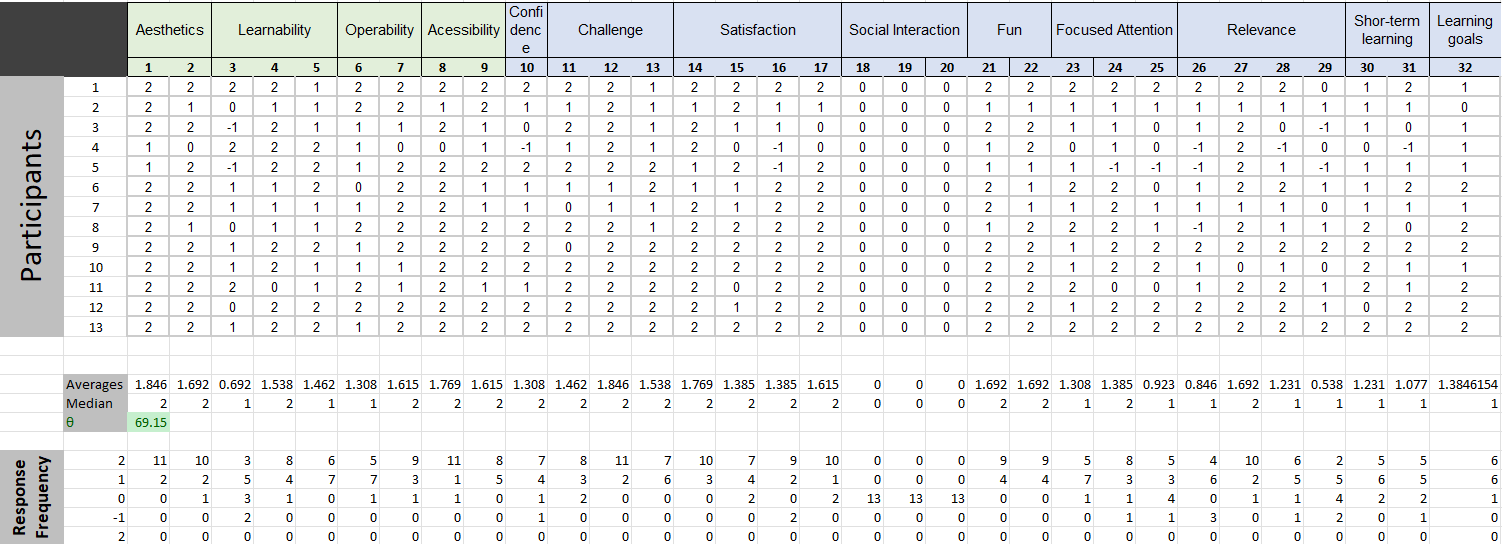
\includegraphics[width=600px,height=300px, angle=270]{Appendices/MeegaAnalysis.png}



%%%%%%%%%%%%%%%%%%%%%%%%%%%%%%%%%%%%%%%%%%%%%%%%%%%%%%%%%%%%%%%%%%%%%%%%%%%%%%%%%%%%%%%%%%%%%%%%%%%%%%
%
%   Filename    : references.tex 
%
%   Description : This file will contain your list of references.
%                 
%%%%%%%%%%%%%%%%%%%%%%%%%%%%%%%%%%%%%%%%%%%%%%%%%%%%%%%%%%%%%%%%%%%%%%%%%%%%%%%%%%%%%%%%%%%%%%%%%%%%%%

\chapter{References}
\label{sec:References}

\sloppy
\begin{adjustwidth}{0.1in}{0.1in}
Alzheimer's Research UK. (2020, March 13). Sea Hero Quest. Retrieved from https://www.alzheimersresearchuk.org/research/for-researchers/resources-and-information/sea-hero-quest/. 

American Physical Society. (October 2008). October 1958: Physicist Invents First Video Game. Retrieved from https://www.aps.org/publications/apsnews/200810/physicshistory.cfm

Bergonse, R. (2017). Fifty Years on, What exactly is a video game? An essentialistic definitional approach. The Computer Games Journal,6(4), 239–255. Retrieved from
https://doi.org/10.1007/s40869-017-0045-4

Colorado College. (2020). Bloom’s Revised Taxonomy. Retrieved from https://www.coloradocollege.edu/other/assessment/how-to-assess-learning/learning-outcomes/blooms-revised-taxonomy.html

Counter-Strike: Global Offensive. [Video game]. (2012). Valve Corporation

Department of Education. (2019). K to 12 Basic Education Curriculum Senior High School - Science, Technology, Engineering and Mathematics (STEM) Specialized Subject Retrieved from https://www.deped.gov.ph/wp-content/uploads/2019/01/Pre-Calculus.pdf

Department of Education. (2018). PISA 2018 National Report of the Philippines. Retrieved from https://www.deped.gov.ph/wp-content/uploads/2019/12/PISA-2018-Philippine-National-Report.pdf.

DOTA 2. [Video game]. (2013). Valve Corporation 


Erik Hazzard (2020, November 5). Data Visualization in games. GameAnalytics. Retrieved from https://gameanalytics.com/blog/data-visualization-games/. 

Gamelearn. (2020, November 13). Serious games examples that explain all you need to know. Retrieved from https://www.game-learn.com/all-you-need-to-know-serious-games-game-based-learning-examples/. 

Gleim Aviation. (2021). X-Plane Flight Training Course. Retrieved from https://www.gleimaviation.com/xplane/

Jaudinez, A. S. (2019). Teaching Senior High School Mathematics: Problems and Interventions. Pedagogical Research, 4(2), em0031. Retrieved from 
https://doi.org/10.29333/pr/5779

Kamnardsiri, T., Hongsit, L.-on, Khuwuthyakorn, P., Wongta, N. (2017). The Effectiveness of the Game-Based Learning System for the Improvement of American Sign Language using Kinect. Retrieved from https://files.eric.ed.gov/fulltext/EJ1154946.pdf. 

Kauffmann, Archava, Castles, Ries, Sullivan, Urquidi, P. S. R. H. S. K. (2011). FACTORS IMPACTING POOR PERFORMANCE IN PRE CALCULUS. Retrieved from https://www.asee.org/file\_server/papers/attachment/file/0001/0803/Pre\_calculus \\ \_ASEE\_2011\_021611.pdfroolvink

Laamarti, F., Eid, M., El Saddik, A. (2014, October 15). An Overview of Serious Games. International Journal of Computer Games Technology. Retrieved from https://www.hindawi.com/journals/ijcgt/2014/358152/

League of Legends (PC version) [Video game]. (2013). Riot Games Inc.

Litts, B., Ramirez, D. (2014). Making people fail: Failing to learn through games and making. Proceedings GLS, 10(2014), 160-166.

Magsambol, B. (2020, December 12). PH lowest among 58 countries in math, science – global assessment. Rappler. Retrieved from https://www.rappler.com/nation/filipino-students-lagging-behind-math-science-timms-international-results-2019. 

Mestadi, W. (2018). An Assessment of Serious Games Technology: Toward an Architecture for Serious Games Design. Retrieved from https://www.hindawi.com/journals/ijcgt/2018/9834565/

Organization for Economic Co-operation and Development. (2018). Programme For International Student Assessment (PISA) Results From PISA 2018. Retrieved from https://www.oecd.org/pisa/publications/PISA2018\_CN\_PHL.pdf.

Plass, J., Homer, B., Kinzer, C. (2015). Foundations of Game-Based Learning. Retrieved from https://files.eric.ed.gov/fulltext/EJ1090277.pdf

Rebbah, H.B.. (2019). The educational effectiveness of serious games. Retrieved from \burl{https://www.researchgate.net/publication/337367093\_The\_educational\_effectiveness\_of\_serious\_games}

Roolvink, F. (2021, March 18). What are serious games? Grendel Games. Retrieved from https://grendelgames.com/what-are-serious-games/

Schoenau-Fog, H. (2011). The Player Engagement Process - An Exploration of Continuation Desire in Digital Games. Retrieved from  http://digra.org/wp-content/uploads/digital-library/11307.06025.pdf

Sharek, D. (2018, September 12). The importance of player engagement. Medium. Retrieved from https://medium.com/horizonperformance/the-importance-of-player-engagement-e424bddc9e87. 

Shute, V., Ke, F.. (2012). Games, Learning, and Assessment. Retrieved from https://www.researchgate.net/publication/283395597\_Games\_Learning\_ \\ and\_Assessment

Sison, R.C., Espulgar, C., Madrigal, L., OBEDOZA, J.B., ROMBLON, N. (2018). Toward an Outcome-Based Methodology for Developing Game-Based Learning Environments. Retrieved from http://icce2018.ateneo.edu/wp-content/uploads/2018/12/C5-11.pdf

Stiller, K. D., Schworm, S. (2019, February 19). Game-Based Learning of the Structure and Functioning of Body Cells in a Foreign Language: Effects on Motivation, Cognitive Load, and Performance.  Retrieved from https://www.frontiersin.org/articles/10.3389/feduc.2019.00018/full\#h4.

Valorant (PC version) [Video game]. (2020). Riot Games Inc.

World Without Oil. (n.d.). Learn About :: World Without Oil. Retrieved from http://writerguy.com/wwo/metaabout.htm. 

Zammitto, V. (2008). Visualization Techniques in Video Games. Retrieved from http://www.sfu.ca/~vzammitt/papers/zammitto-EVA-Visualization\_Techniques\_in\_VideoGames.pdf
\end{adjustwidth}
\fussy

%\bibliographystyle{apacite}       %-- specified APA style for bibliograpy
                                  %-- more details about APA style citation can be found in www.ctan.org/tex-archive/biblio/bibtex/contrib/apacite/

                                  %-- bibliographic entries are handled via bibtex; refer to www.bibtex.org for more details


%%%%%%%%%%%%%%%%%%%%%%%%%%%%%%%%%%%%%%%%%%%%%%%%%%%%%%%%%%%%%%%%%%%%%%%%%%%%%%%%%%%%%%%%%%%%%%%%%%%%%%%
%
%   Filename    : references.tex 
%
%   Description : This file will contain your list of references.
%                 
%%%%%%%%%%%%%%%%%%%%%%%%%%%%%%%%%%%%%%%%%%%%%%%%%%%%%%%%%%%%%%%%%%%%%%%%%%%%%%%%%%%%%%%%%%%%%%%%%%%%%%

\chapter{References}
\label{sec:References}

\sloppy
\begin{adjustwidth}{0.1in}{0.1in}
Alzheimer's Research UK. (2020, March 13). Sea Hero Quest. Retrieved from https://www.alzheimersresearchuk.org/research/for-researchers/resources-and-information/sea-hero-quest/. 

American Physical Society. (October 2008). October 1958: Physicist Invents First Video Game. Retrieved from https://www.aps.org/publications/apsnews/200810/physicshistory.cfm

Bergonse, R. (2017). Fifty Years on, What exactly is a video game? An essentialistic definitional approach. The Computer Games Journal,6(4), 239–255. Retrieved from
https://doi.org/10.1007/s40869-017-0045-4

Colorado College. (2020). Bloom’s Revised Taxonomy. Retrieved from https://www.coloradocollege.edu/other/assessment/how-to-assess-learning/learning-outcomes/blooms-revised-taxonomy.html

Counter-Strike: Global Offensive. [Video game]. (2012). Valve Corporation

Department of Education. (2019). K to 12 Basic Education Curriculum Senior High School - Science, Technology, Engineering and Mathematics (STEM) Specialized Subject Retrieved from https://www.deped.gov.ph/wp-content/uploads/2019/01/Pre-Calculus.pdf

Department of Education. (2018). PISA 2018 National Report of the Philippines. Retrieved from https://www.deped.gov.ph/wp-content/uploads/2019/12/PISA-2018-Philippine-National-Report.pdf.

DOTA 2. [Video game]. (2013). Valve Corporation 


Erik Hazzard (2020, November 5). Data Visualization in games. GameAnalytics. Retrieved from https://gameanalytics.com/blog/data-visualization-games/. 

Gamelearn. (2020, November 13). Serious games examples that explain all you need to know. Retrieved from https://www.game-learn.com/all-you-need-to-know-serious-games-game-based-learning-examples/. 

Gleim Aviation. (2021). X-Plane Flight Training Course. Retrieved from https://www.gleimaviation.com/xplane/

Jaudinez, A. S. (2019). Teaching Senior High School Mathematics: Problems and Interventions. Pedagogical Research, 4(2), em0031. Retrieved from 
https://doi.org/10.29333/pr/5779

Kamnardsiri, T., Hongsit, L.-on, Khuwuthyakorn, P., Wongta, N. (2017). The Effectiveness of the Game-Based Learning System for the Improvement of American Sign Language using Kinect. Retrieved from https://files.eric.ed.gov/fulltext/EJ1154946.pdf. 

Kauffmann, Archava, Castles, Ries, Sullivan, Urquidi, P. S. R. H. S. K. (2011). FACTORS IMPACTING POOR PERFORMANCE IN PRE CALCULUS. Retrieved from https://www.asee.org/file\_server/papers/attachment/file/0001/0803/Pre\_calculus \\ \_ASEE\_2011\_021611.pdfroolvink

Laamarti, F., Eid, M., El Saddik, A. (2014, October 15). An Overview of Serious Games. International Journal of Computer Games Technology. Retrieved from https://www.hindawi.com/journals/ijcgt/2014/358152/

League of Legends (PC version) [Video game]. (2013). Riot Games Inc.

Litts, B., Ramirez, D. (2014). Making people fail: Failing to learn through games and making. Proceedings GLS, 10(2014), 160-166.

Magsambol, B. (2020, December 12). PH lowest among 58 countries in math, science – global assessment. Rappler. Retrieved from https://www.rappler.com/nation/filipino-students-lagging-behind-math-science-timms-international-results-2019. 

Mestadi, W. (2018). An Assessment of Serious Games Technology: Toward an Architecture for Serious Games Design. Retrieved from https://www.hindawi.com/journals/ijcgt/2018/9834565/

Organization for Economic Co-operation and Development. (2018). Programme For International Student Assessment (PISA) Results From PISA 2018. Retrieved from https://www.oecd.org/pisa/publications/PISA2018\_CN\_PHL.pdf.

Plass, J., Homer, B., Kinzer, C. (2015). Foundations of Game-Based Learning. Retrieved from https://files.eric.ed.gov/fulltext/EJ1090277.pdf

Rebbah, H.B.. (2019). The educational effectiveness of serious games. Retrieved from \burl{https://www.researchgate.net/publication/337367093\_The\_educational\_effectiveness\_of\_serious\_games}

Roolvink, F. (2021, March 18). What are serious games? Grendel Games. Retrieved from https://grendelgames.com/what-are-serious-games/

Schoenau-Fog, H. (2011). The Player Engagement Process - An Exploration of Continuation Desire in Digital Games. Retrieved from  http://digra.org/wp-content/uploads/digital-library/11307.06025.pdf

Sharek, D. (2018, September 12). The importance of player engagement. Medium. Retrieved from https://medium.com/horizonperformance/the-importance-of-player-engagement-e424bddc9e87. 

Shute, V., Ke, F.. (2012). Games, Learning, and Assessment. Retrieved from https://www.researchgate.net/publication/283395597\_Games\_Learning\_ \\ and\_Assessment

Sison, R.C., Espulgar, C., Madrigal, L., OBEDOZA, J.B., ROMBLON, N. (2018). Toward an Outcome-Based Methodology for Developing Game-Based Learning Environments. Retrieved from http://icce2018.ateneo.edu/wp-content/uploads/2018/12/C5-11.pdf

Stiller, K. D., Schworm, S. (2019, February 19). Game-Based Learning of the Structure and Functioning of Body Cells in a Foreign Language: Effects on Motivation, Cognitive Load, and Performance.  Retrieved from https://www.frontiersin.org/articles/10.3389/feduc.2019.00018/full\#h4.

Valorant (PC version) [Video game]. (2020). Riot Games Inc.

World Without Oil. (n.d.). Learn About :: World Without Oil. Retrieved from http://writerguy.com/wwo/metaabout.htm. 

Zammitto, V. (2008). Visualization Techniques in Video Games. Retrieved from http://www.sfu.ca/~vzammitt/papers/zammitto-EVA-Visualization\_Techniques\_in\_VideoGames.pdf
\end{adjustwidth}
\fussy       %-- the file "myreferences.bib" is a sample bibliography (bib) from SIGGRAPH 
                                  %-- your job: **CREATE/EDIT** your own bibliography file  

\end{document}

